\section{Statistical Analysis}
\label{sec:analysis:method}



Having carried out the event selection as described in section~\ref{sec:analysis:selection}, the estimation of the \PW branching fraction is carried out using two different approaches.  Before describing the two approaches, it will be useful to describe the formalism that is common to both.



%%%%%%%%%%%%%%%%%%%%%%%%%%%%%%%%%%%%%%%%
% 1. Determination of Signal Acceptance
%%%%%%%%%%%%%%%%%%%%%%%%%%%%%%%%%%%%%%%%
\subsection{Modeling the Decays of WW Pairs}
\label{sec:analysis:method:effMatrix}


The quantities of interest are the four \PW branching fractions,
\begin{equation}
    \vbw = \{\bwe, \bwm, \bwt, \bwh\},
\end{equation}
\noindent where the subscript indicates the decay mode of the \PW boson (hadronic decay modes, h, are grouped together).  Because the $\PGt$ can also decay to the other modes, the above vector can be extended to include this,
\begin{equation}
    \vbw^\prime = \{\bwe, \bwm, \bwt\bte, \bwt\btm, \bwt\bth, \bwh\}.
\end{equation}
\noindent Because this analysis is interested in final states with two \PW bosons, it is necessary to consider all possible decay combinations.  This can be represented succinctly in matrix representation by taking the outer product of $\vbw^\prime$ with itself,
\begin{equation}
\label{eqn:analysis:method:effMatrix:br_matrix}
    \boldsymbol{B} =  \vbw^\prime\otimes \vbw^\prime =
    \begin{bmatrix}
        \bwe \bwe       & \bwe \bwm         & \bwe \bwt \bte        & \bwe \bwt \btm        & \bwe \bwt \bth        & \bwe \bwh         \\
        \bwm \bwe       & \bwm \bwm         & \bwm \bwt \bte        & \bwm \bwt \btm        & \bwm \bwt \bth        & \bwm \bwh         \\
        \bwt \bte \bwe  & \bwt \bte \bwm    & \bwt \bte \bwt \bte   & \bwt \bte \bwt \btm   & \bwt \bte \bwt \bth   & \bwt \bte \bwh    \\
        \bwt \btm \bwe  & \bwt \btm\bwm     & \bwt \btm \bwt \bte   & \bwt \btm \bwt \btm   & \bwt \btm \bwt \bth   & \bwt \btm \bwh    \\
        \bwt \bth \bwe  & \bwt \bth \bwm    & \bwt \bth \bwt \bte   & \bwt \bth \bwt \btm   & \bwt \bth \bwt \bth   & \bwt \bth \bwh    \\
        \bwh \bwe       & \bwh \bwm         & \bwh \bwt \bte        & \bwh \bwt \btm        & \bwh \bwt \bth        & \bwh  \bwh 
	\end{bmatrix}
    . 
\end{equation}
\noindent This is a 36 term symmetric matrix containing 21 unique terms. The signal samples are constructed from a combination of \ttbar and \tW final states, and are divided into 21 categories based on the decay modes identified by inspecting generator-level truth information.  The efficiencies for these signal samples can be summarized in matrix notation,
\begin{equation}
\label{eqn:analysis:method:effMatrix:eff_matrix}
    \boldsymbol{E} = \begin{bmatrix}
        \epsilon_{\Pe\Pe}       & \epsilon_{\Pe\PGm}        & \epsilon_{\Pe\PGte}       & \epsilon_{\Pe\PGtmu}          & \epsilon_{\Pe\PGth}       & \epsilon_{\Pe \mathrm{h}}   \\
        \epsilon_{\Pe\PGm}      & \epsilon_{\PGm\PGm}       & \epsilon_{\PGm\PGte}      & \epsilon_{\PGm\PGtmu}         & \epsilon_{\PGm\PGth}      & \epsilon_{\PGm \mathrm{h}}  \\
        \epsilon_{\Pe\PGte}     & \epsilon_{\PGm\PGte}      & \epsilon_{\PGte\PGte}     & \epsilon_{\PGte\PGtmu}        & \epsilon_{\PGte\PGth}     & \epsilon_{\PGte \mathrm{h}} \\
        \epsilon_{\Pe\PGtmu}    & \epsilon_{\PGm\PGtmu}     & \epsilon_{\PGte\PGtmu}    & \epsilon_{\PGtmu\PGtmu}       & \epsilon_{\PGtmu\PGth}    & \epsilon_{\PGtmu \mathrm{h}}\\
        \epsilon_{\Pe\PGth}     & \epsilon_{\PGm\PGth}      & \epsilon_{\PGte\PGth}     & \epsilon_{\PGtmu\PGth}        & \epsilon_{\PGth\PGth}     & \epsilon_{\PGth \mathrm{h}} \\
        \epsilon_{\Pe\mathrm{h}}& \epsilon_{\PGm\mathrm{h}} & \epsilon_{\PGte\mathrm{h}}& \epsilon_{\PGtmu\mathrm{h}}   & \epsilon_{\PGth\mathrm{h}}& \epsilon_\mathrm{hh}        \\
    \end{bmatrix},
\end{equation}
\noindent where the subscript on the $\PGt$ indicates its decay mode.  This matrix is constructed for each signal process in each channel and $n_j n_\PQb$ category, and, in the case of the shape analysis, the fitted \pt observable.  The value of the efficiencies are calculated based on the ratio,
\begin{equation}
\label{eqn:analysis:method:effMatrix:model_eff}
    \epsilon_{ij} = \frac{\sum_{k}w_{ij}^k}{N^{\rm gen}_{ij}},
\end{equation}
\noindent where $w^{k}$ is the weight for event $k$ and $N_{gen}$ is the total number of events generated for a given process.  Based on this, the estimated number of events for a signal process, $s$, that produces two \PW bosons can be written,
\begin{equation}
\label{eqn:analysis:method:effMatrix:data_model}
    N_{s} = \sigma_{s} L \boldsymbol{E}_{s,ij} \Bij ,
\end{equation}
\noindent where $\sigma_{s}$ is the cross-section for process under consideration, $L$ is the integrated luminosity.  Having established these preliminaries, the particulars of the twoanalysis approaches will be described in detail in the next two sections.
\FloatBarrier






%%%%%%%%%%%%%%%%%%%%%%%%%%%%%%%%%%%%%%%%
% 2. Shape analysis
%%%%%%%%%%%%%%%%%%%%%%%%%%%%%%%%%%%%%%%%

\subsection{Shape Analysis}
\label{sec:analysis:method:mle}

In this approach, a maximum likelihood estimation of the branching fractions is carried out.  The data is divided into categories based on the multiplicity and flavor of leptons, jet multiplicity, and \PQb tag multiplicities as described in section~\ref{sec:analysis:event}.  Additional discriminating information is included by further binning the data according to a single kinematic observable in each category category. The observable is selected to enhance the discrimination between decay products that come directly from the \PW boson decay and decay products where a tau lepton is an intermediate product.  The variables that are selected by each lepton flavor category are as follows:
\begin{itemize}
    \item \cee, \cmm, \cem: the trailing lepton \pt
    \item \cet and \cmt: the hadronic tau \pt
    \item \ceh and \cmh: the triggering lepton \pt
\end{itemize}
\noindent These distributions are shown in Figures~\ref{fig:analysis:method:mle:fits_templates_ll} through \ref{fig:analysis:method:mle:fit_templates_l4j}. Histogram templates are generated for each category by binning using the Bayesian Block algorithm~\cite{Pollack:2017srh}.  The binning is calculated independently for each category based on $\sim 10^{4}$ simulated events.
\begin{figure}[htb!]
    \centering
    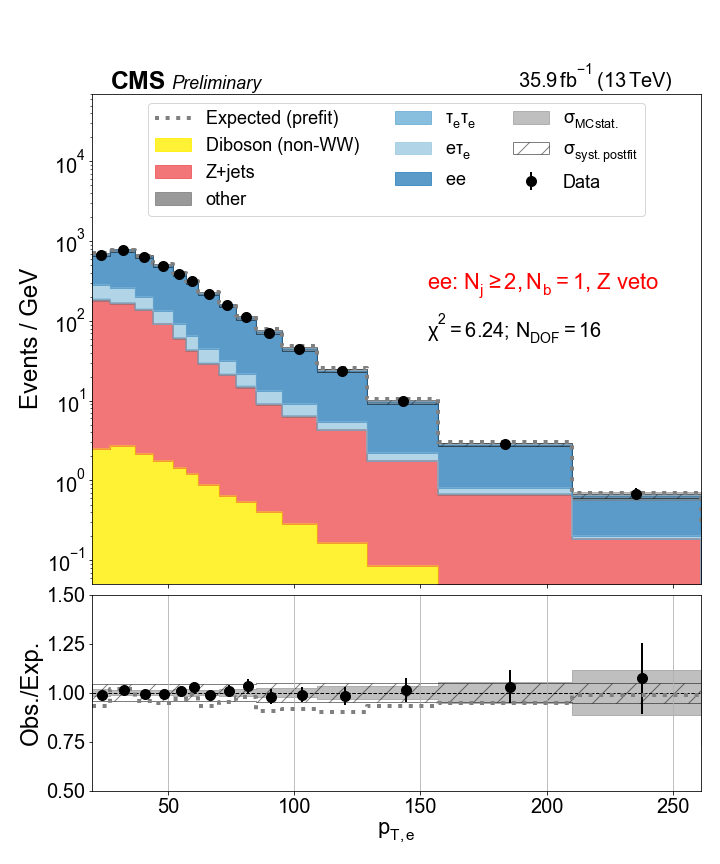
\includegraphics[width=0.35\textwidth]{chapters/Analysis/sectionStatisticalAnalysis/figures/fit/ee_cat_gt2_eq1_b}
    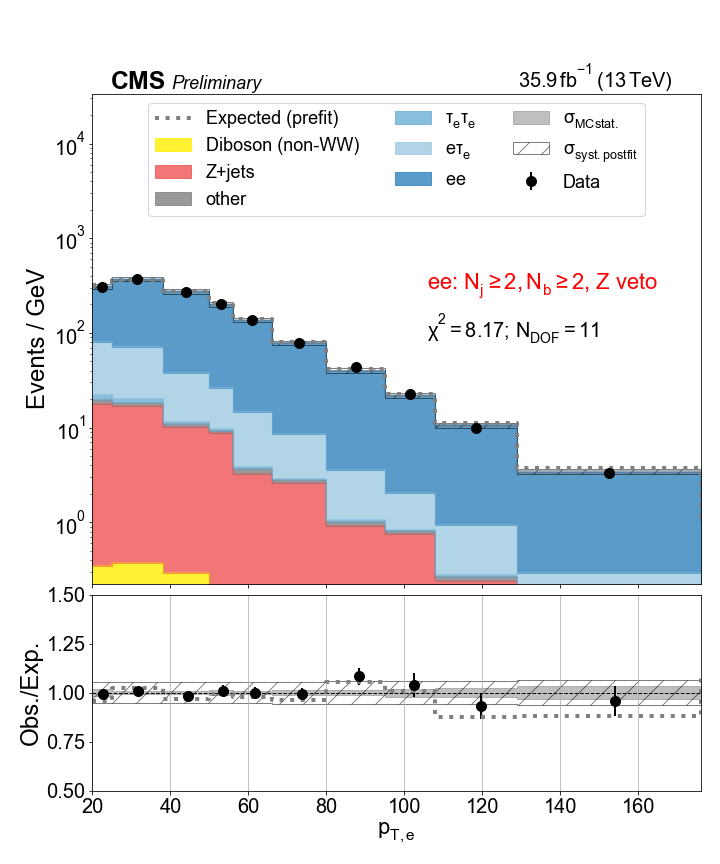
\includegraphics[width=0.35\textwidth]{chapters/Analysis/sectionStatisticalAnalysis/figures/fit/ee_cat_gt2_gt2_b}
    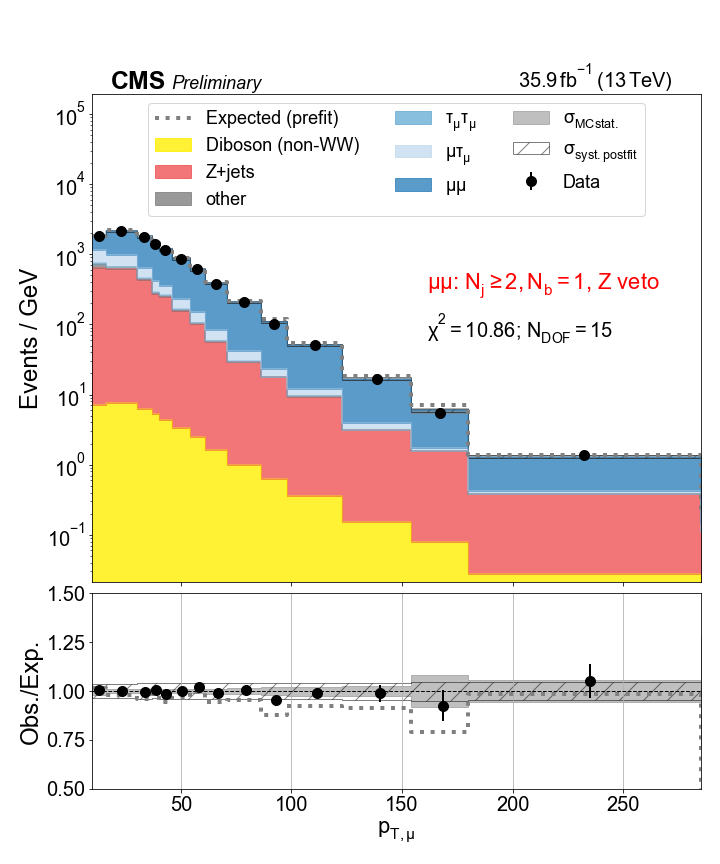
\includegraphics[width=0.35\textwidth]{chapters/Analysis/sectionStatisticalAnalysis/figures/fit/mumu_cat_gt2_eq1_b}
    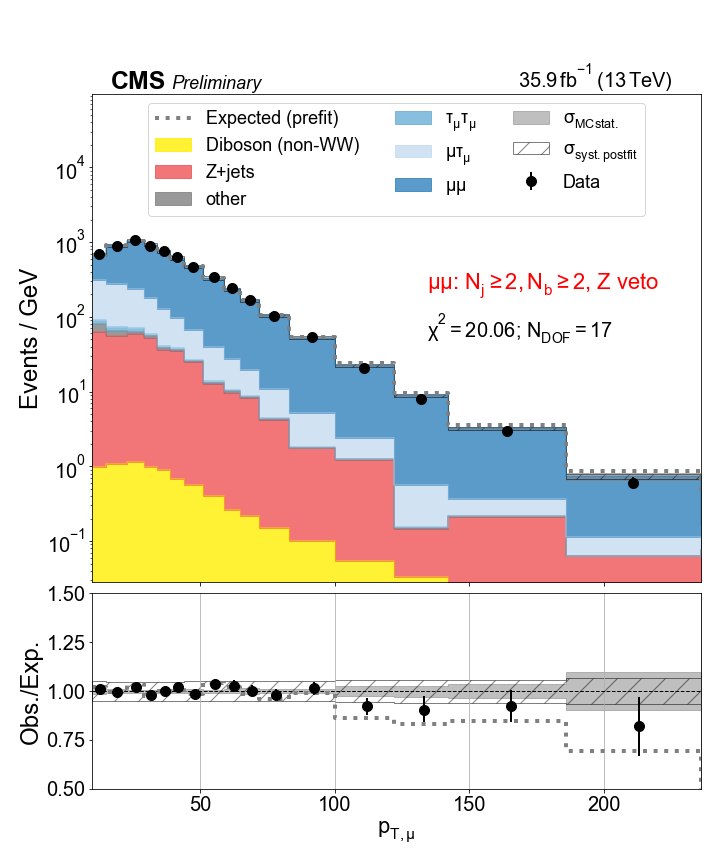
\includegraphics[width=0.35\textwidth]{chapters/Analysis/sectionStatisticalAnalysis/figures/fit/mumu_cat_gt2_gt2_b}
    \caption{Templates used as inputs to the fit for the \cee and \cmm channels.}
    \label{fig:analysis:method:mle:fits_templates_ll}
\end{figure}
\begin{figure}[htb!]
    \centering
    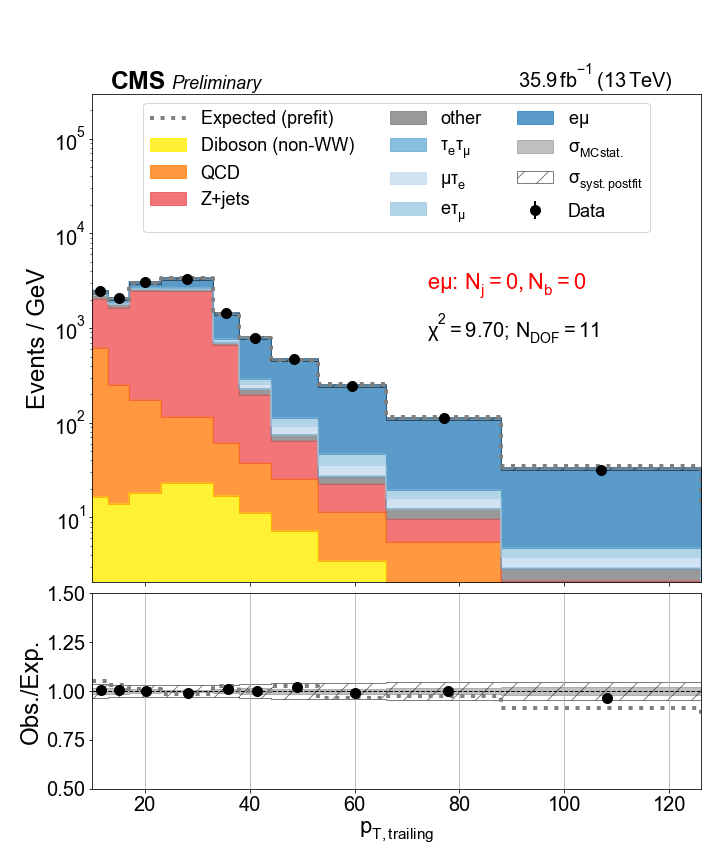
\includegraphics[width=0.3\textwidth]{chapters/Analysis/sectionStatisticalAnalysis/figures/fit/emu_cat_eq0_eq0_a}
    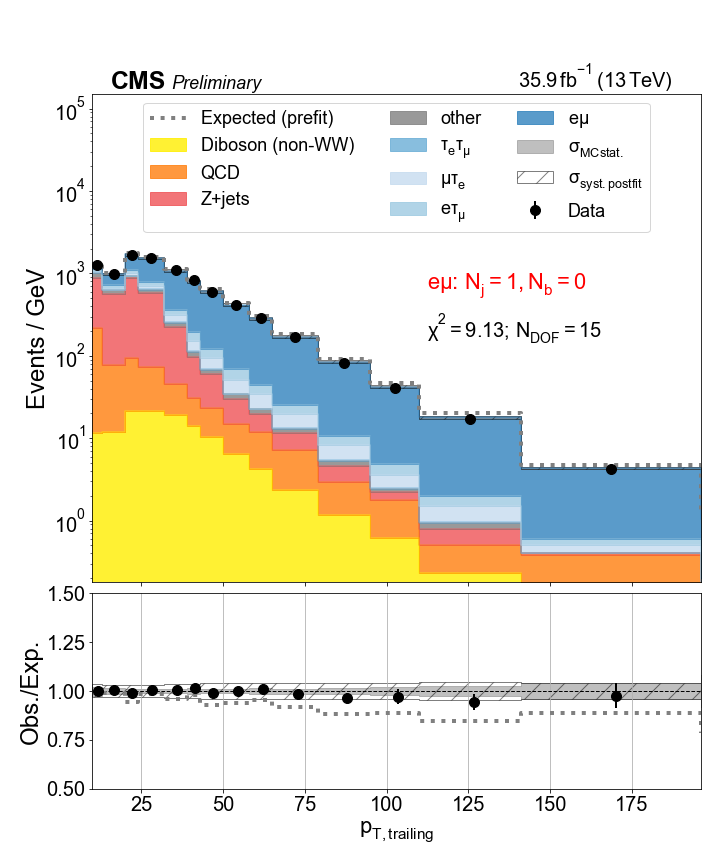
\includegraphics[width=0.3\textwidth]{chapters/Analysis/sectionStatisticalAnalysis/figures/fit/emu_cat_eq1_eq0_a}
    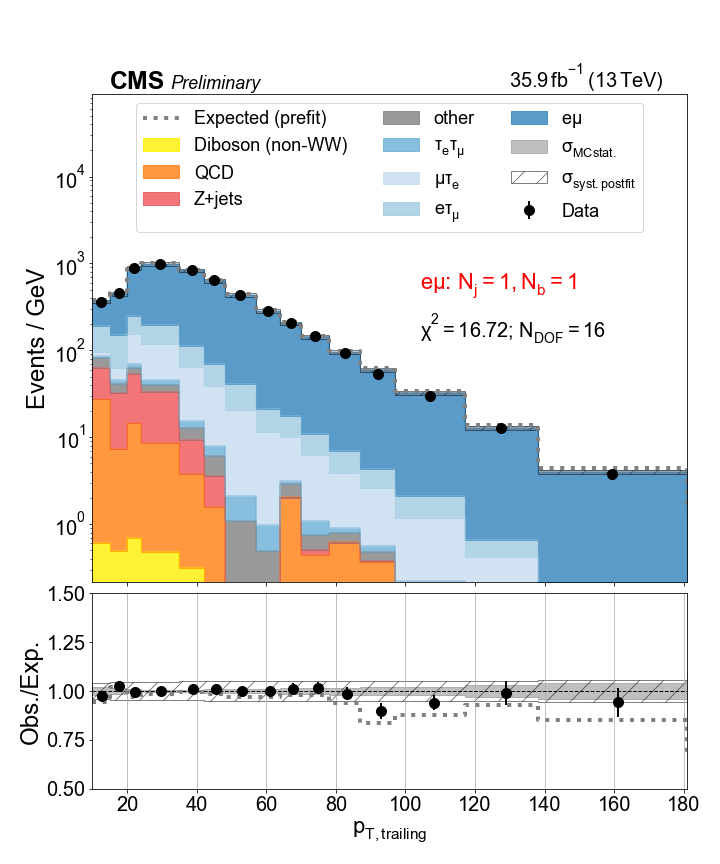
\includegraphics[width=0.3\textwidth]{chapters/Analysis/sectionStatisticalAnalysis/figures/fit/emu_cat_eq1_eq1_a}

    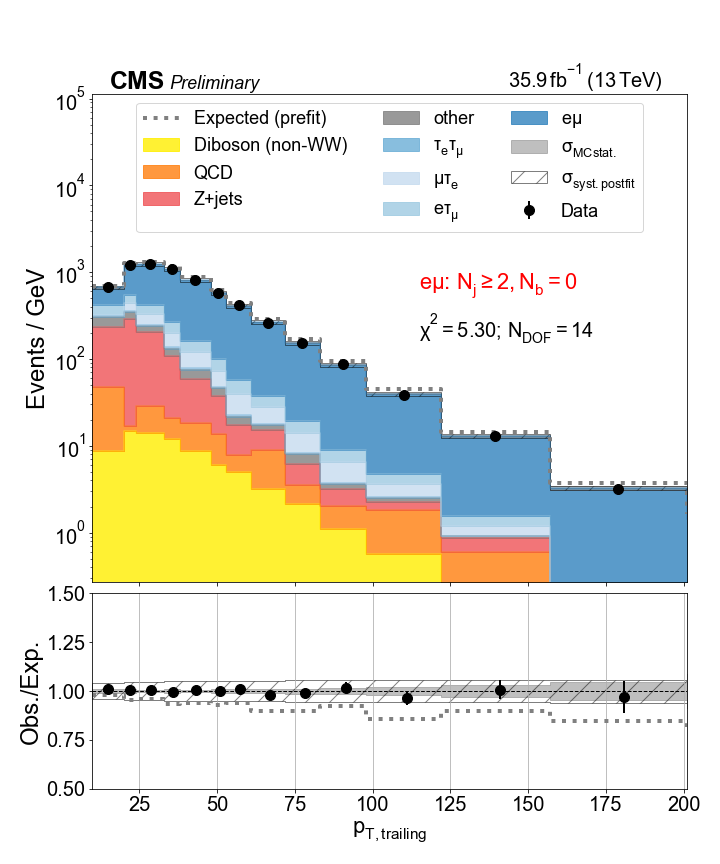
\includegraphics[width=0.3\textwidth]{chapters/Analysis/sectionStatisticalAnalysis/figures/fit/emu_cat_gt2_eq0}
    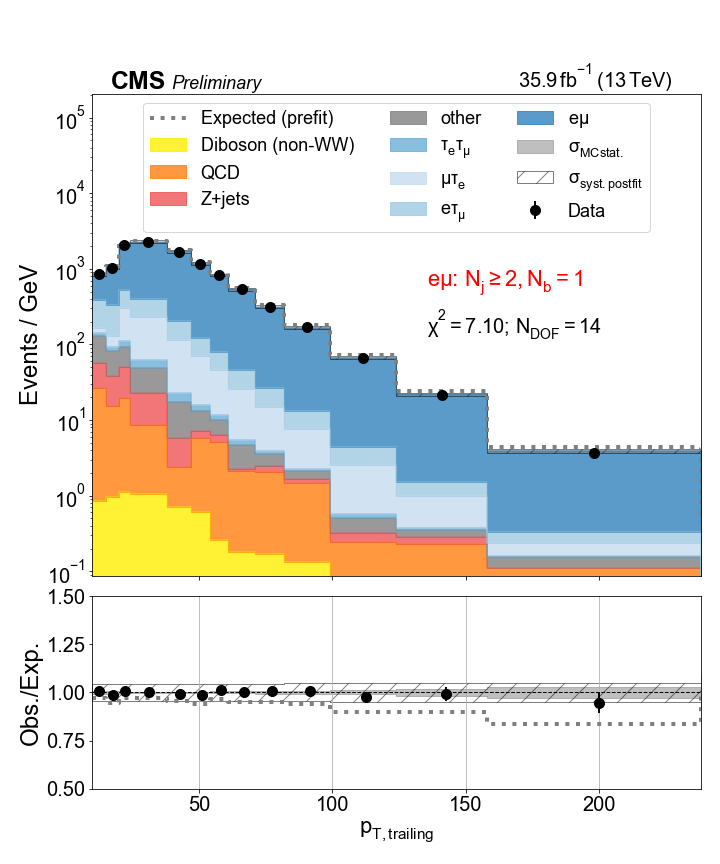
\includegraphics[width=0.3\textwidth]{chapters/Analysis/sectionStatisticalAnalysis/figures/fit/emu_cat_gt2_eq1_a}
    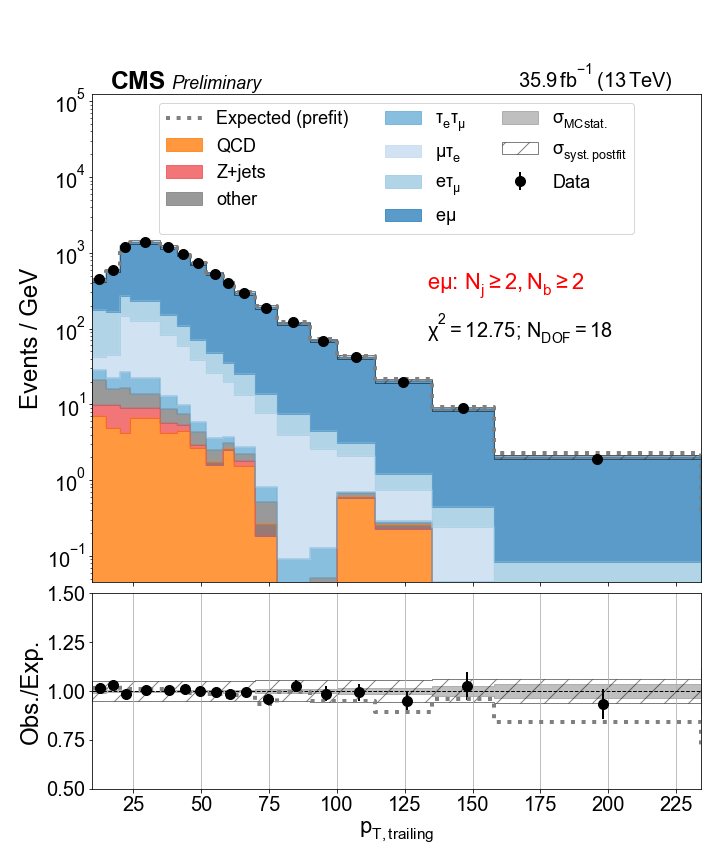
\includegraphics[width=0.3\textwidth]{chapters/Analysis/sectionStatisticalAnalysis/figures/fit/emu_cat_gt2_gt2_a}
    \caption{Templates used as inputs to the fit for the \cem channel.}
    \label{fig:analysis:method:mle:fits_templates_emu}
\end{figure}
\begin{figure}[htb!]
    \centering
    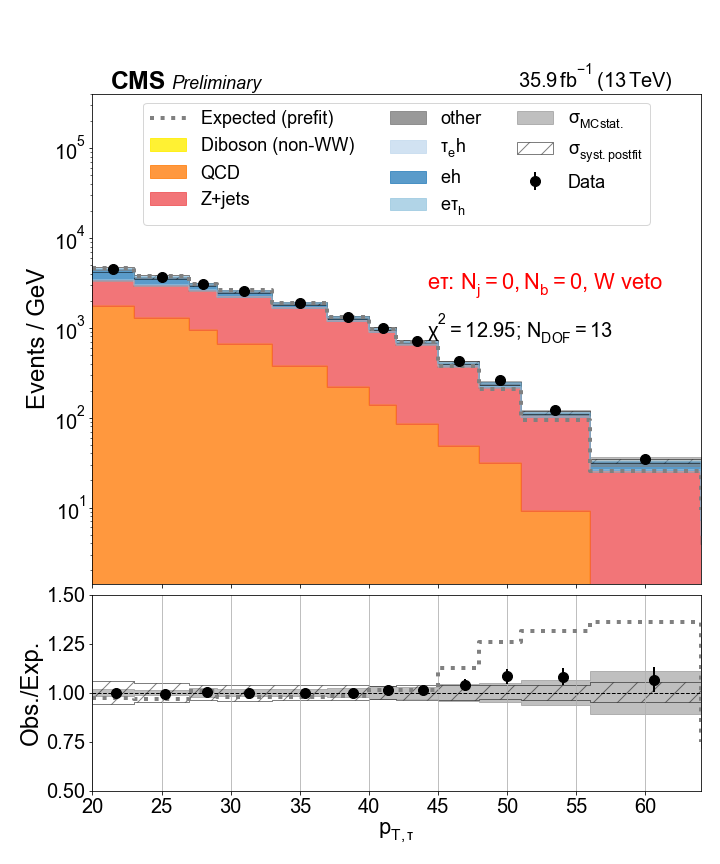
\includegraphics[width=0.24\textwidth]{chapters/Analysis/sectionStatisticalAnalysis/figures/fit/etau_cat_eq0_eq0}
    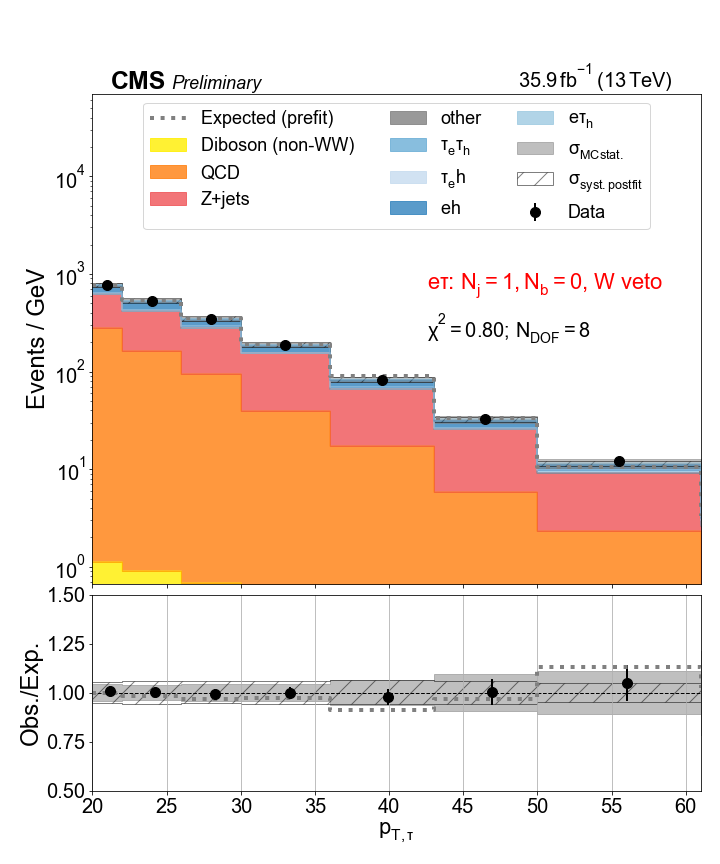
\includegraphics[width=0.24\textwidth]{chapters/Analysis/sectionStatisticalAnalysis/figures/fit/etau_cat_eq1_eq0}
    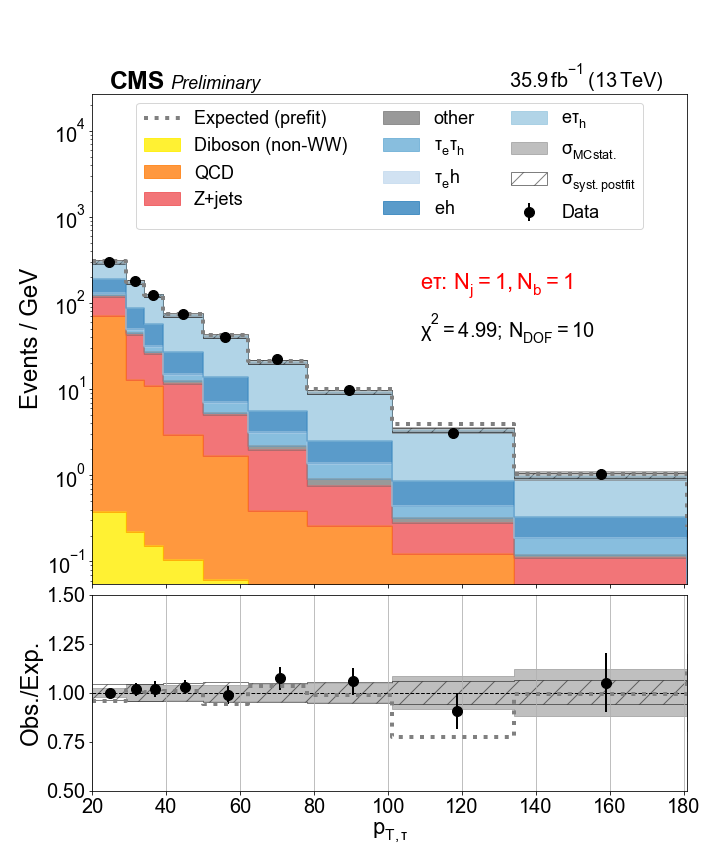
\includegraphics[width=0.24\textwidth]{chapters/Analysis/sectionStatisticalAnalysis/figures/fit/etau_cat_eq1_eq1}
    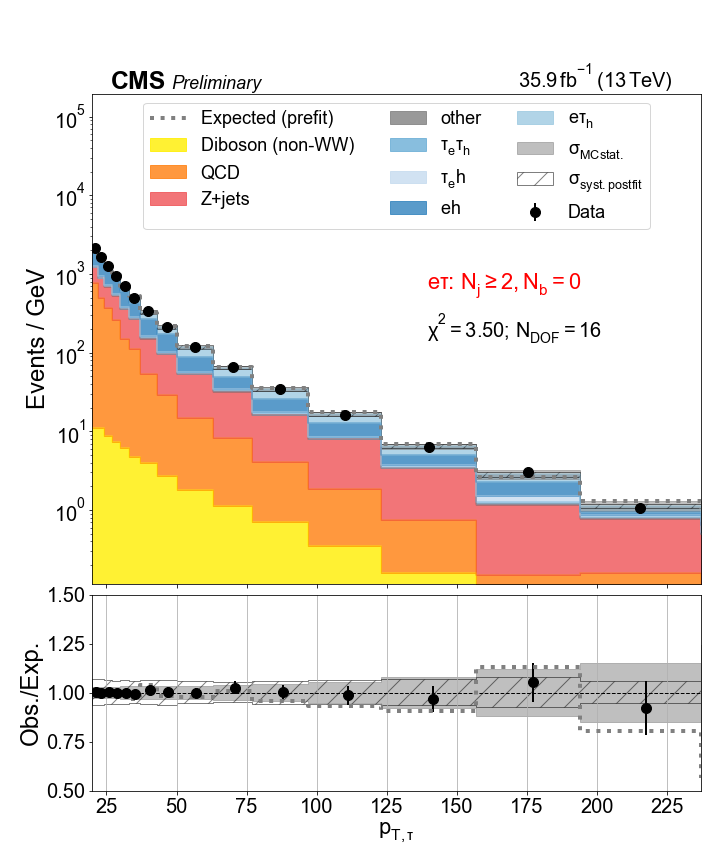
\includegraphics[width=0.24\textwidth]{chapters/Analysis/sectionStatisticalAnalysis/figures/fit/etau_cat_gt2_eq0}

    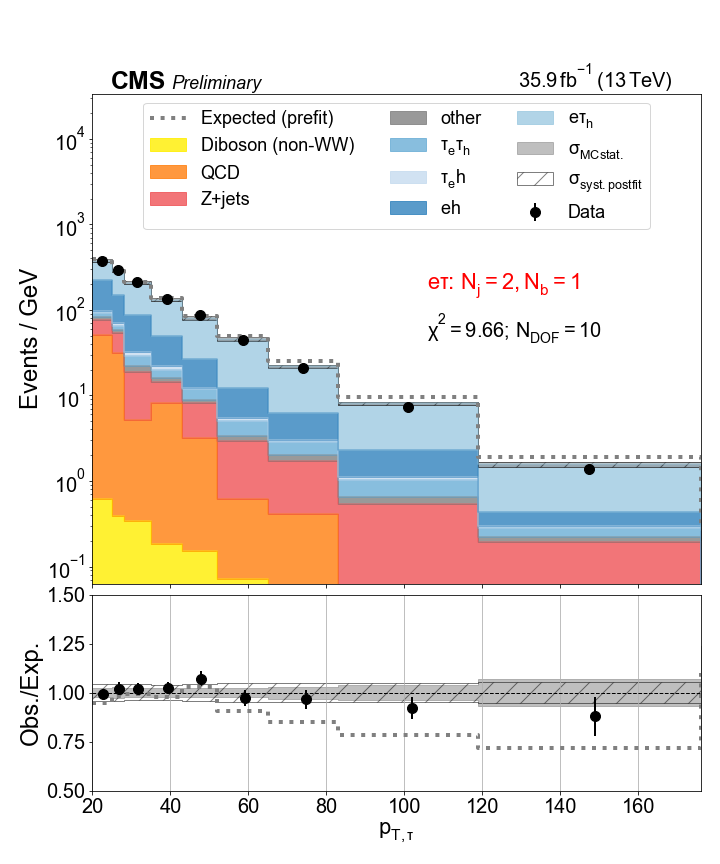
\includegraphics[width=0.24\textwidth]{chapters/Analysis/sectionStatisticalAnalysis/figures/fit/etau_cat_eq2_eq1}
    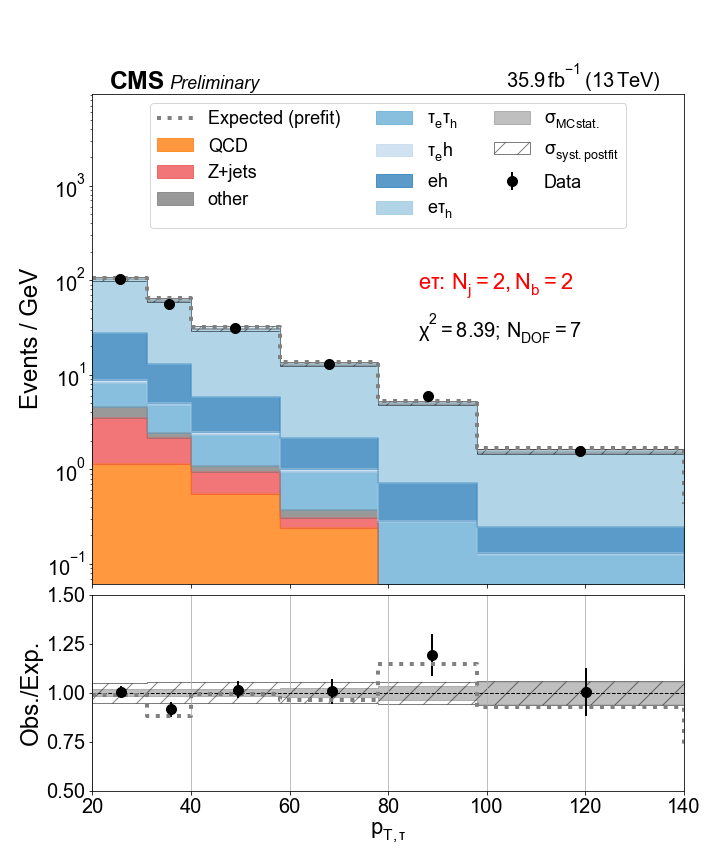
\includegraphics[width=0.24\textwidth]{chapters/Analysis/sectionStatisticalAnalysis/figures/fit/etau_cat_eq2_eq2}
    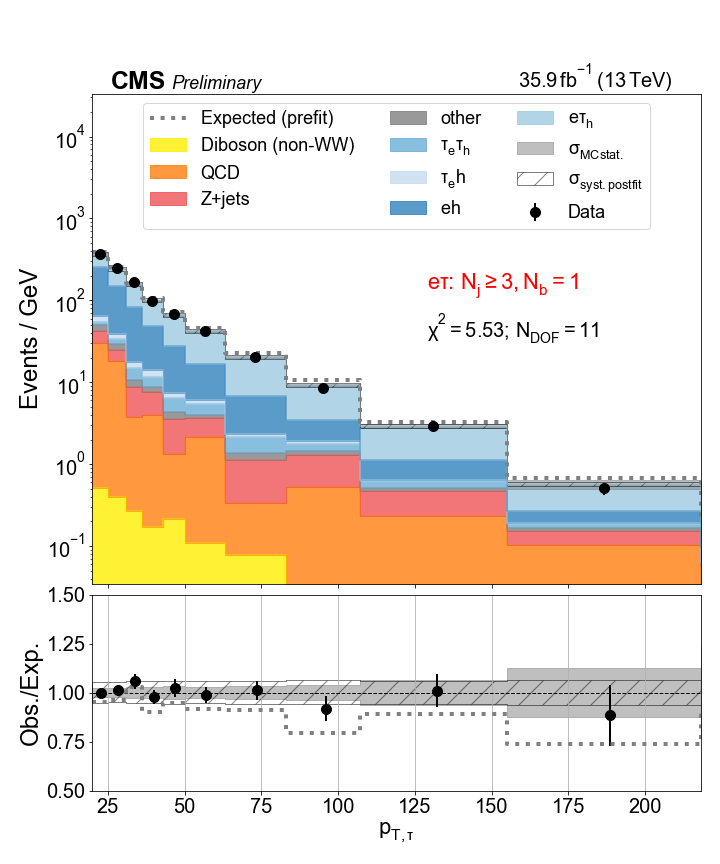
\includegraphics[width=0.24\textwidth]{chapters/Analysis/sectionStatisticalAnalysis/figures/fit/etau_cat_gt3_eq1}
    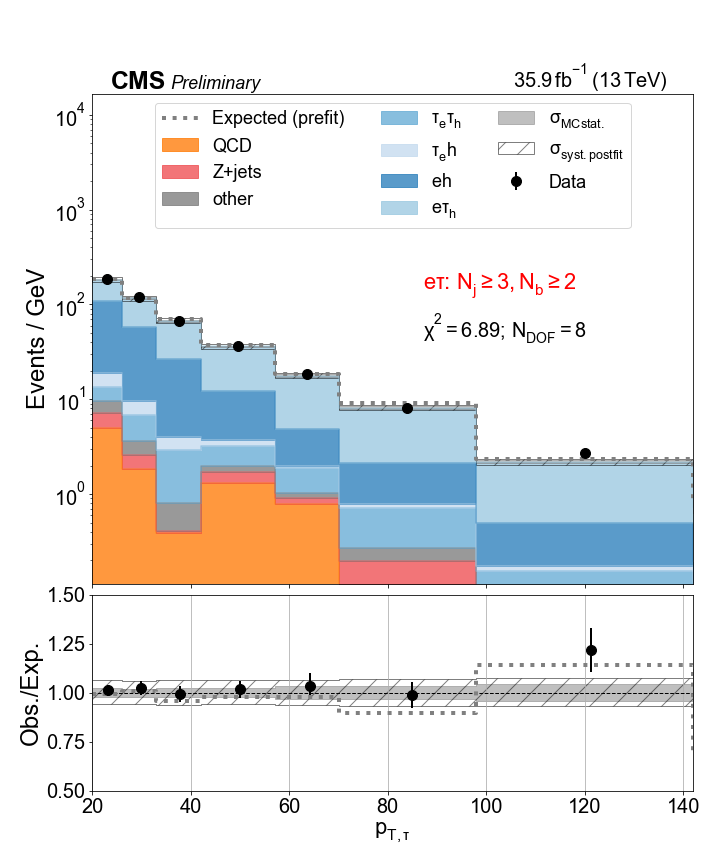
\includegraphics[width=0.24\textwidth]{chapters/Analysis/sectionStatisticalAnalysis/figures/fit/etau_cat_gt3_gt2}
    \caption{Templates used as inputs to the fit for the \cet channel.}
    \label{fig:analysis:method:mle:fits_templates_etau}
\end{figure}
\begin{figure}[htb!]
    \centering
    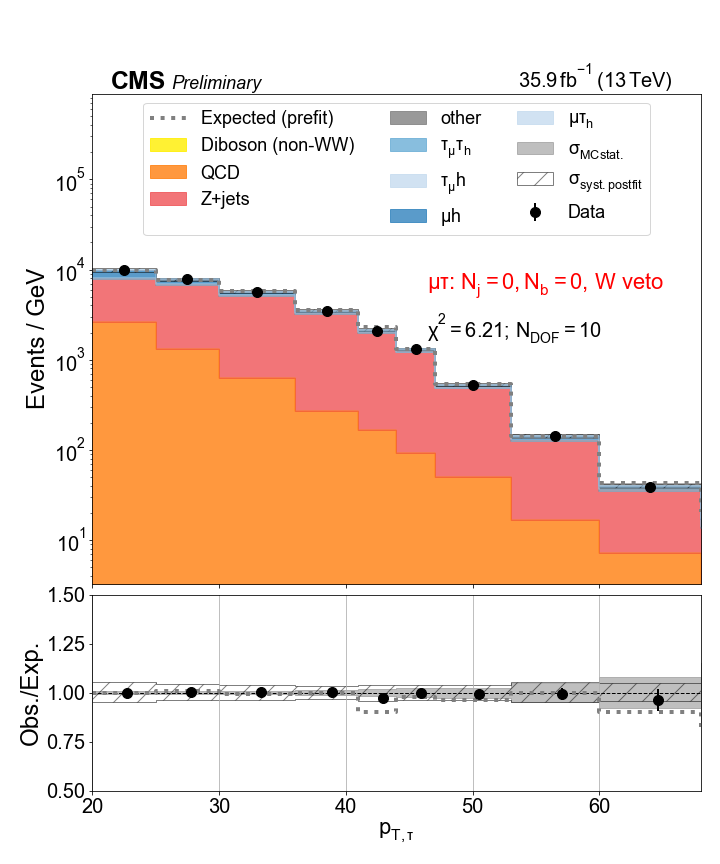
\includegraphics[width=0.24\textwidth]{chapters/Analysis/sectionStatisticalAnalysis/figures/fit/mutau_cat_eq0_eq0}
    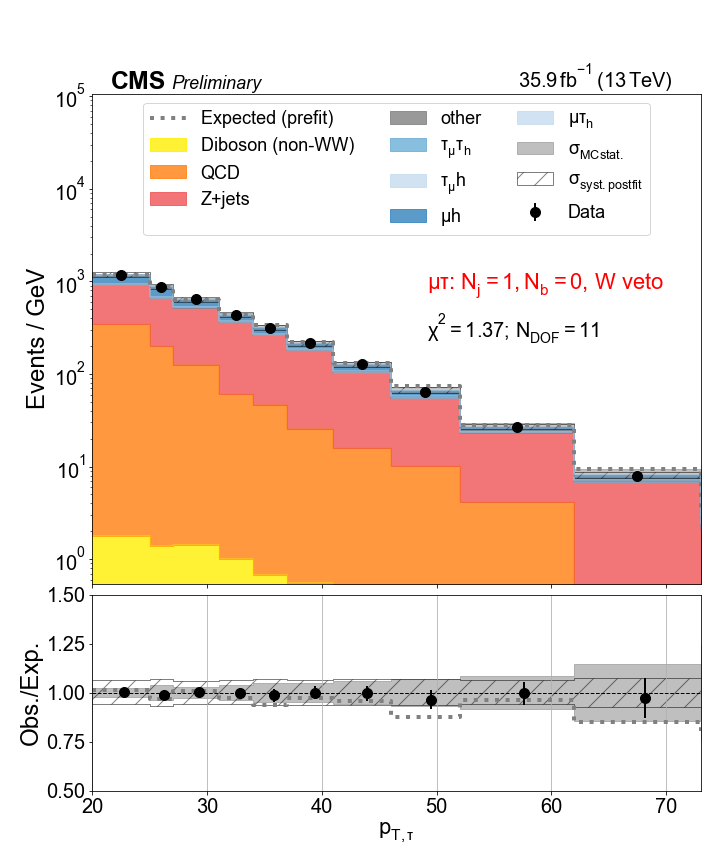
\includegraphics[width=0.24\textwidth]{chapters/Analysis/sectionStatisticalAnalysis/figures/fit/mutau_cat_eq1_eq0}
    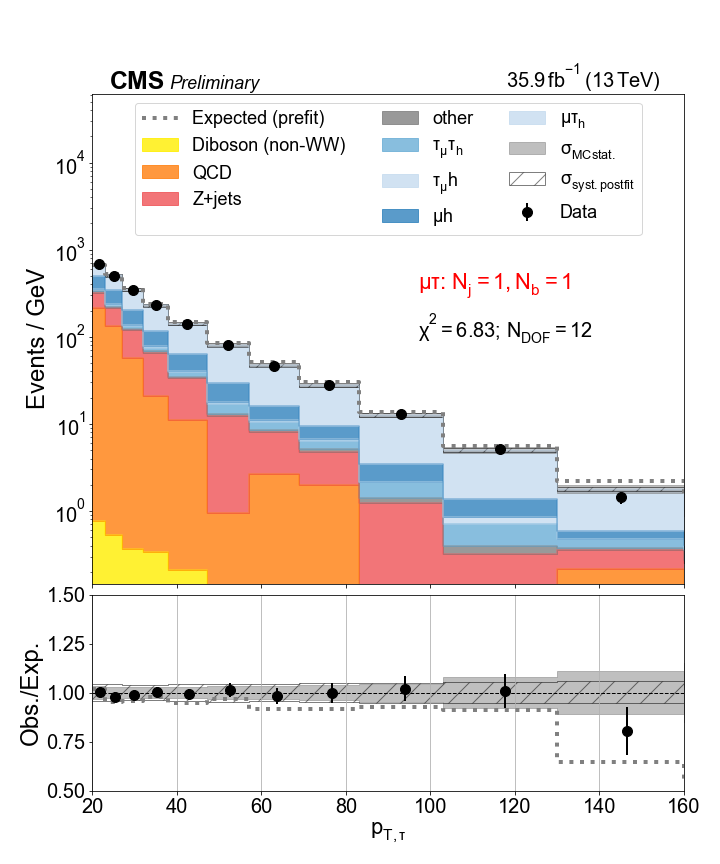
\includegraphics[width=0.24\textwidth]{chapters/Analysis/sectionStatisticalAnalysis/figures/fit/mutau_cat_eq1_eq1}
    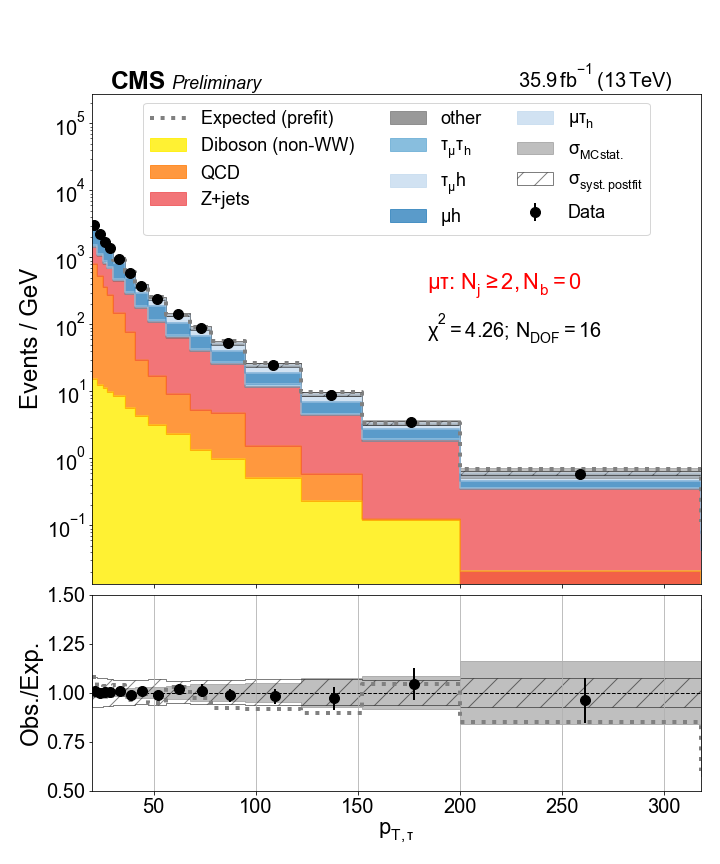
\includegraphics[width=0.24\textwidth]{chapters/Analysis/sectionStatisticalAnalysis/figures/fit/mutau_cat_gt2_eq0}

    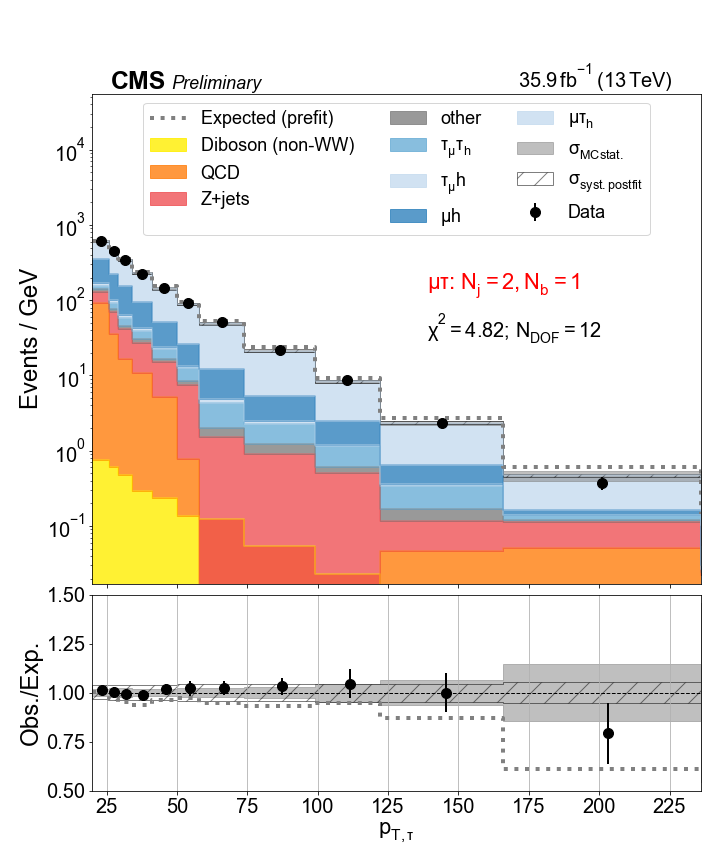
\includegraphics[width=0.24\textwidth]{chapters/Analysis/sectionStatisticalAnalysis/figures/fit/mutau_cat_eq2_eq1}
    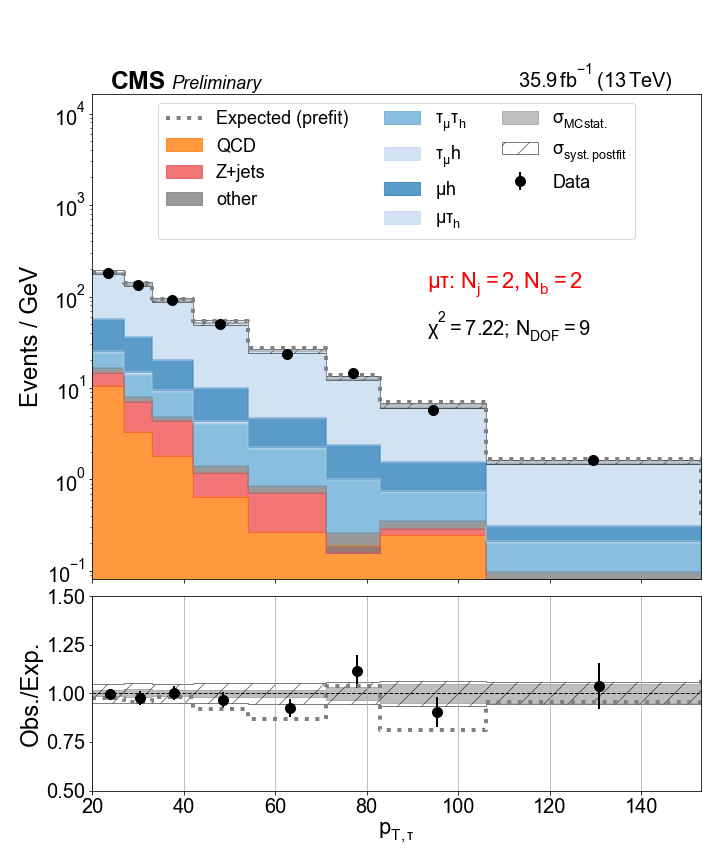
\includegraphics[width=0.24\textwidth]{chapters/Analysis/sectionStatisticalAnalysis/figures/fit/mutau_cat_eq2_eq2}
    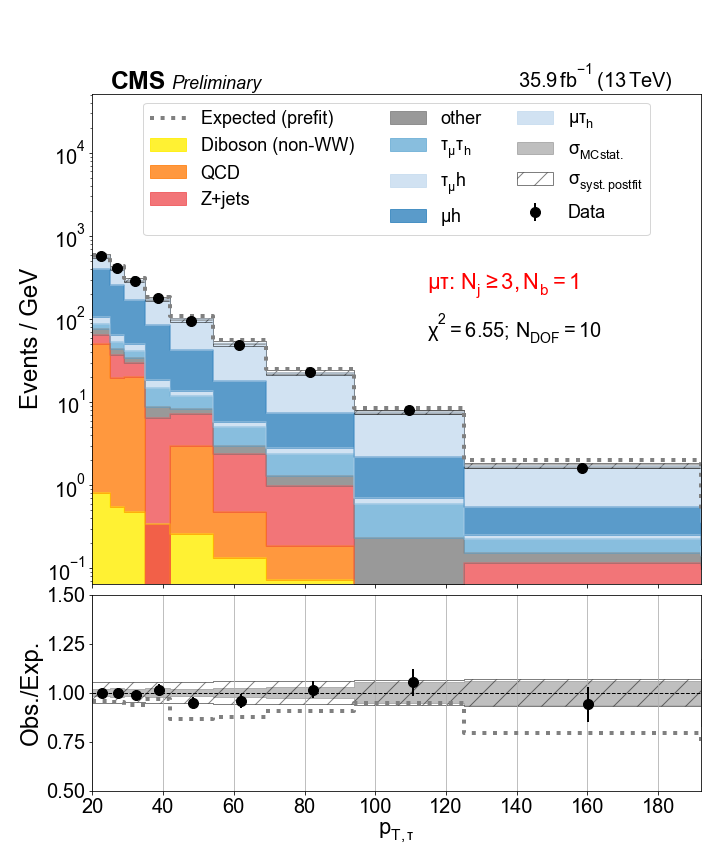
\includegraphics[width=0.24\textwidth]{chapters/Analysis/sectionStatisticalAnalysis/figures/fit/mutau_cat_gt3_eq1}
    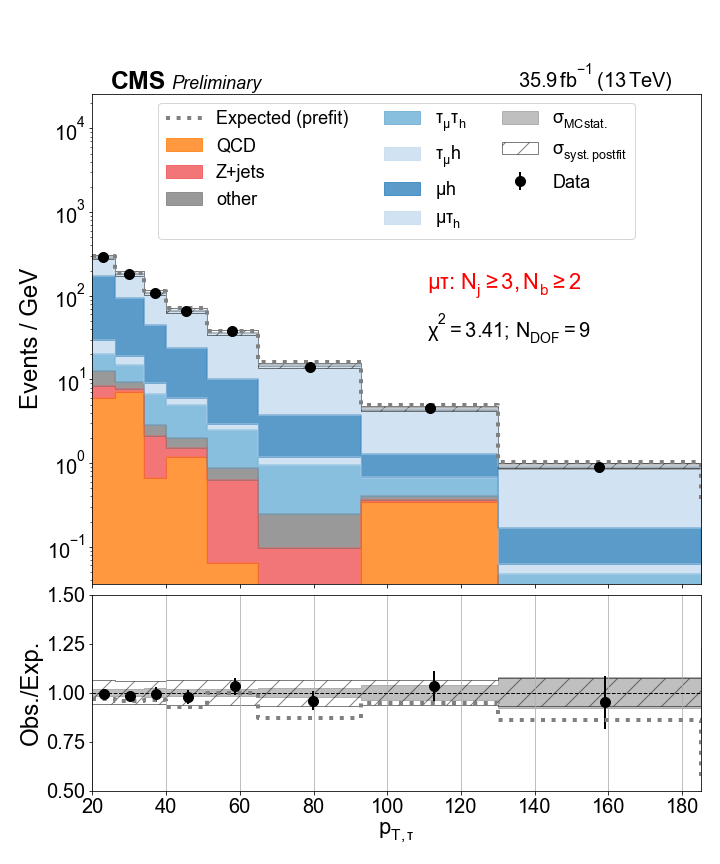
\includegraphics[width=0.24\textwidth]{chapters/Analysis/sectionStatisticalAnalysis/figures/fit/mutau_cat_gt3_gt2}
    \caption{Templates used as inputs to the fit for the \cmt channel.}
    \label{fig:analysis:method:mle:fits_templates_mutau}
\end{figure}
\begin{figure}[htb!]
    \centering
    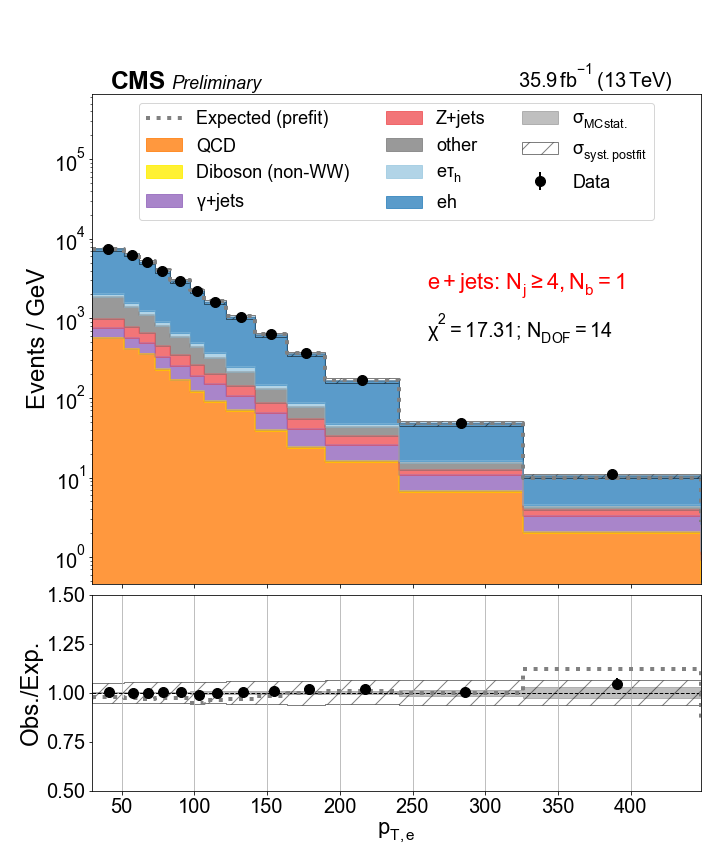
\includegraphics[width=0.35\textwidth]{chapters/Analysis/sectionStatisticalAnalysis/figures/fit/ejet_cat_gt4_eq1}
    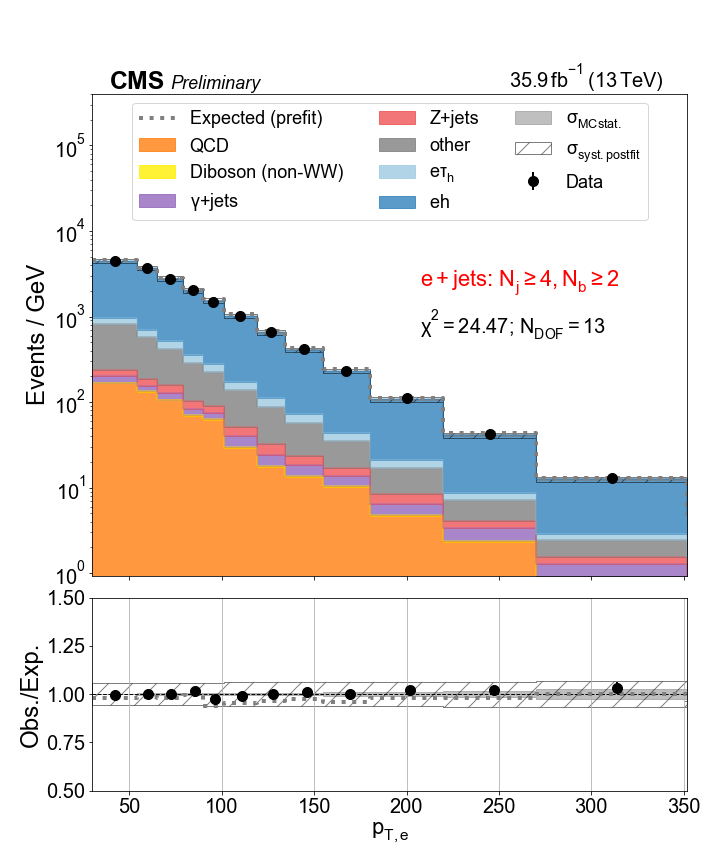
\includegraphics[width=0.35\textwidth]{chapters/Analysis/sectionStatisticalAnalysis/figures/fit/ejet_cat_gt4_gt2}
    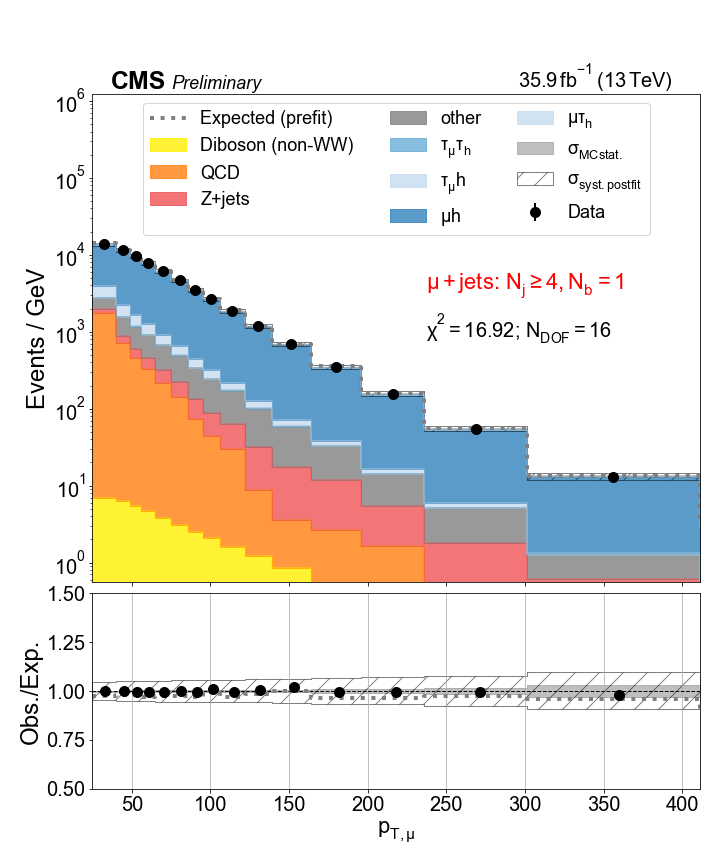
\includegraphics[width=0.35\textwidth]{chapters/Analysis/sectionStatisticalAnalysis/figures/fit/mujet_cat_gt4_eq1}
    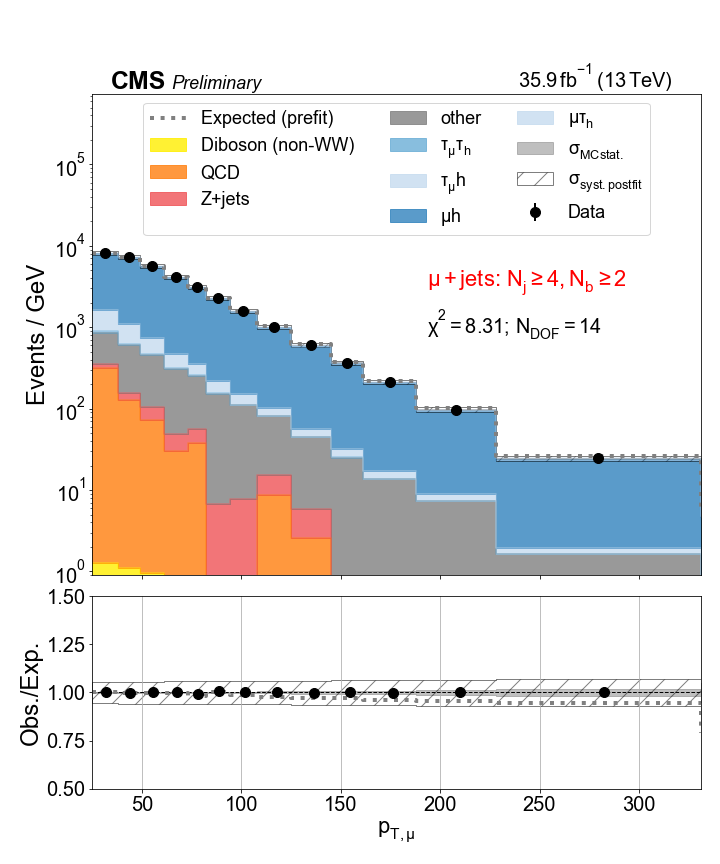
\includegraphics[width=0.35\textwidth]{chapters/Analysis/sectionStatisticalAnalysis/figures/fit/mujet_cat_gt4_gt2}
    \caption{Templates used as inputs to the fit for the \ceh and \cmh channels.}
    \label{fig:analysis:method:mle:fit_templates_l4j}
\end{figure}



Effectively, this parameterizes the efficiency matrix in Equation~\ref{eqn:analysis:method:effMatrix:eff_matrix} by the observables listed above, the number of jets, and the number of \PQb tags.  Having constructed the data model, the negative log likelihood can be constructed,
\begin{equation}
\label{eqn:analysis:method:mel_nll}
    NLL(\vbw) = \sum_{\mathrm{i\in bin}} \left[ - y_{i}\ln f_{i}(\vbw) + f_{i}(\vbw) \right],
\end{equation}
\noindent where $y_{i}$ is the data yield in bin $i$.  The predicted yields, $f_{i}$ are a sum of signal and background templates, 
\begin{equation}
    f(\vbw) = \sum_{\rm sig.}s(\vbw) + \sum_{\rm bkg.} b.
\end{equation}
\noindent where the signal term, $s(\vbw)$ is as written in Equation~\ref{eqn:analysis:method:effMatrix:data_model} and the background term $b$ is estimated by either simulated dataset or data driven approach described in Section~\ref{sec:analysis:background}.



\subsubsection{Assessment of Systematic Uncertainties}
\label{sec:analysis:shape_syst}

The shape analysis accounts for the effects of various sources of systematic uncertainties by incorporating nuisance parameters into the fit~\cite{Conway:2011in}.  The individual sources of systematics uncertainties are described in section~\ref{sec:analysis:systematics}.  This approach to the systematic uncertainties has the benefit that all correlations between the various nuisance parameters that exist in the model definition are accounted for when the regression is carried out.  In some cases, the nuisance parameters can become constrained by the fit.  Additionally, it is straight forward to incorporate auxiliary control regions ($\PZ\to\PGtl\PGth$) to improve the constraints on background normalizations and uncertainties on the modeling of physics objects in simulation.

The modification to the objective function follows the approach recommended by Conway, i.e., adding additional terms, $\pi(\vnp)$, to the cost function to account for the priors on the nuisance parameters, $\theta$,
\begin{equation}
\label{eqn:analysis:method:mel_nll_full}
    NLL(\vbw, \vnp) = \sum_{\mathrm{i \in bins}} \left[-y_{i}\ln f_{i}(\vbw, \vnp) + f_{i}(\vbw, \vnp)\right] + \pi(\vnp).
\end{equation}
Nuisance parameters are assumed to be Gaussian constrained unless otherwise noted. Thus the corresponding negative log likelihood term takes the form of L2 regularization $\pi(\vnp) = \frac{1}{2} \abs{\vnp}^2$. In the predictive model $f_{i}(\vbw, \vnp)$, the nuisance parameters are treated either as normalization parameters (multiplicative factors which are bin independent) or shape nuisance parameters which vary depending on the bin they are applied to.  In the latter case, morphing templates are generated for the cases that the nuisance parameters are shifted up and down by one standard deviation. The details for each source of systematic uncertainty is described in section~\ref{sec:analysis:systematics}. A quadratic morphing of the bin content as a function of a nuisance parameter is used for values $\theta \in [-1, 1]$,
\begin{equation}
\label{eqn:analysis:method:shape_param}
    f(\theta) = \frac{\theta(\theta - 1)}{2}f^{-} - (\theta - 1)(\theta +1)f^{0} + \frac{\theta(\theta + 1)}{2}f^{+},
\end{equation}
\noindent with $f^{0}$ corresponding to the nominal prediction in a given bin, and $f^{-}$ and $f^{+}$ correspond to the down and up variations of the relevant source of uncertainty. In the circumstance that the variation in yield is symmetric about nominal value as a function of $\theta$, the quadratic term becomes unimportant.  Outside the range $[-1, 1]$, the bin content varies linearly with the value of $\theta$.
% It is useful to rewrite this expression so the dependence on $\theta$ is clearer,
% \begin{align}
%     \Delta f(\theta) = f(\theta) - f^{0} = \frac{\theta^{2}}{2}(\Delta\epsilon^{+} + \Delta\epsilon^{-}) 
%      + \frac{\theta}{2}(\Delta\epsilon^{+} - \Delta\epsilon^{-}) \\
%      &= \frac{\Delta_{+}}{2}\theta^{2}  + \frac{\Delta_{-}}{2}\theta
% \end{align}

% where,
% \begin{equation}
%     \Delta\epsilon^{\pm} = \epsilon^{\pm} - \epsilon^{0}, \quad \Delta_{\pm} = \Delta\epsilon^{+} \pm \Delta\epsilon^{-} .
% \end{equation}

% It is worth noting that 
% \begin{equation}
%     \Delta\epsilon = 
%     \begin{cases}
%             (\Delta_{+} + \frac{\Delta_{-}}{2})\theta - \frac{\Delta_{+}}{2},
%             & \text{if } \theta > 1 \\
%             (-\Delta_{+} + \frac{\Delta_{-}}{2})\theta - \frac{\Delta_{+}}{2},
%             & \text{if } \theta < -1
%     \end{cases}
% \end{equation}

% This is derived by requiring that $\Delta\epsilon$ be continuous and
% differentiable at the boundaries.  The total change to the predicted
% efficiency is then the sum over all $\Delta\epsilon$, 
% \begin{equation}
%     \epsilon' = \epsilon^{0} + \sum_{\theta\in\vnp}\Delta\epsilon_{\theta}
% \end{equation}

The branching fraction estimates are determined by minimizing the $NLL$ Equation~\ref{eqn:analysis:method:mel_nll_full} with respect to all parameters.  This is done for all final state channels and \PQb tag bins simultaneously which accounts for correlations between common nuisance parameters and the \PW branching fractions.

\subsubsection{Assessment of Statistical Uncertainty}
In addition to various sources of uncertainty associated with the detector and with the modeling of physical processes, there is a non-negligible uncertainty arising from the finite and limited statistics of the simulated samples used to model the data.  Ideally, the simulated samples would have $>5$ times the number of events collected in data for each process.  This is generally not the case, and in some cases, the number of simulated events is less than the number of corresponding events collected in data.  With this in mind, the Barlow-Beeston lite method is adopted to account for the resulting uncertainty.  In brief, this entails introducing a nuisance parameter for each bin in the analysis that controls the normalization of that bin and is constrained according to the variance associated with the statistics of the simulated samples.  Because, these n.p. are to first order not correlated across bins, they can be solved for analytically as described in section 5 of Conway~\cite{Conway:2011in}.

% originally from the systematic uncertainty
This analysis relies heavily on simulated samples to estimate backgrounds and the signal processes.  The number of events generated in each simulated sample is frequently limited so an additional uncertainty must be assessed to account for this.  For the most part, it is not an issue in the counting analysis, but it is still accounted for by varying the MC templates within their statistical uncertainties and carrying out the analysis.  For the shape analysis, the Barlow-Beeston method~\cite{Amsler:2008zzb} is adopted.  This method includes an intermediate step in the minimization of the $NLL$ where the $NLL$ is minimized with respect to nuisance parameters associated with the normalization of individual bins.  The nuisance parameters are allowed to vary within the combined MC statistical uncertainty associated with the bin.  The impact of this is particularly large where the normalization of the Drell-Yan sample is concerned since the size of the simulated sample is on the order of the number of events produced in data.



\subsubsection{Bias Study of Parameter Extraction}

It is desirable that the method produces an unbiased measurement of the \PW branching fractions.  Even though it is not expected that bias should arise, it is worth verifying this with a toy MC study.  This is carried out by generating ten thousand pseudo-datasets from the nominal data model templates with values of the branching fractions samples in the ranges $\bwe, \bwm, \bwt \in [0.1, 0.12]$ with $\bwh = 1 - (\bwe + \bwm + \bwt)$.  For each of the ten thousand quadruplets, a pseudo-dataset is generated accounting for Poisson statistics of each individual signal and background template, and the search procedure is carried out, i.e., Equation~\ref{eqn:analysis:method:mel_nll} is minimized to determine the observed estimator.  From this, the bias can be determined,
\begin{equation}
\label{eqn:analysis:method:mle:bias}
    \mathrm{bias} = \frac{\beta_{\rm true} - \beta_{\rm  obs}}{\beta_{ \rm  true}}.
\end{equation}

The results of this study are shown in figures~\ref{fig:analysis:method:mle:bias_scan} and \ref{fig:analysis:method:mle:bias_test}.  The mean value of the bias shows no deviation from zero within the variance.  There is also no indication that there is a dependence of the bias on the true value of the branching fraction used to generate the data.

\begin{figure}[htb!]
    \centering
    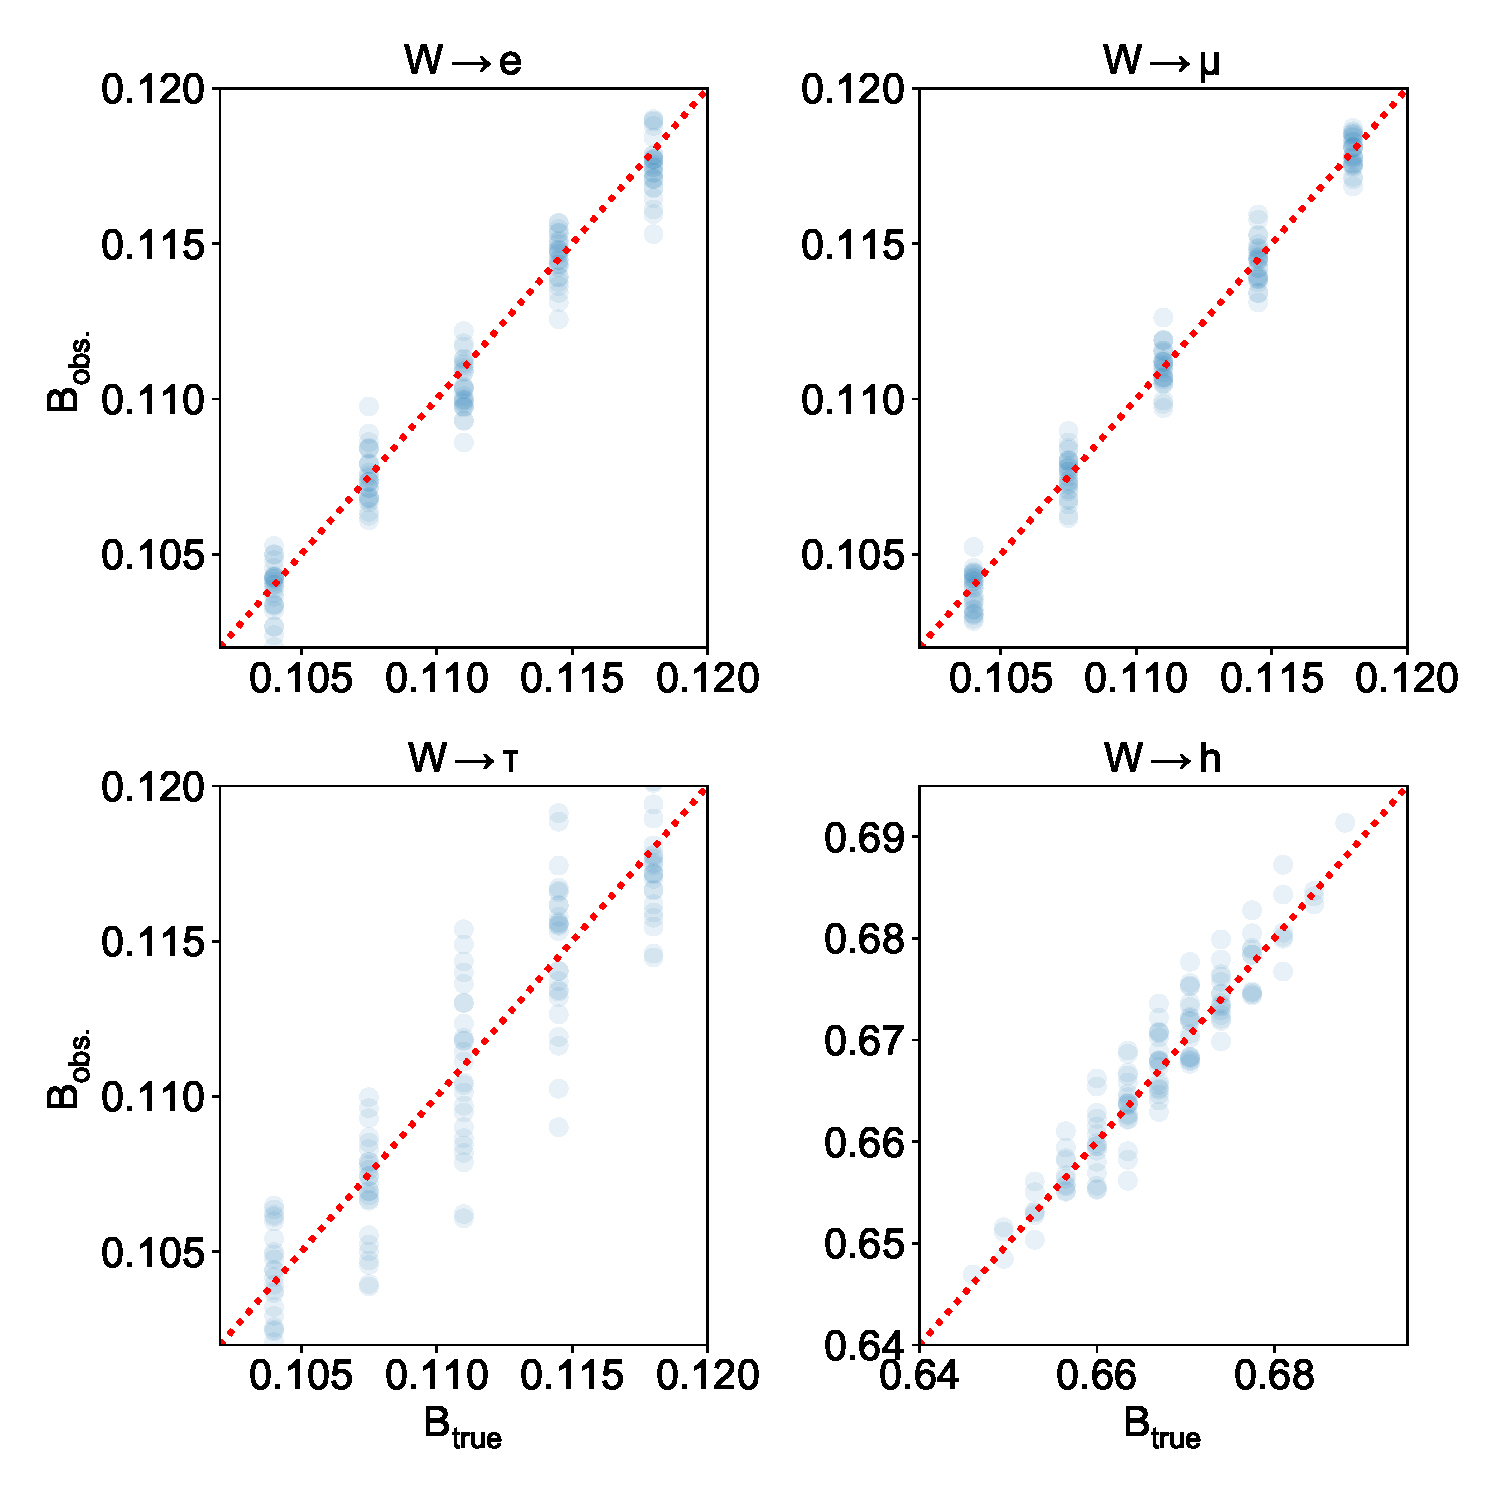
\includegraphics[width=0.7\textwidth]{chapters/Analysis/sectionStatisticalAnalysis/figures/beta_scan}
    \caption{Results of bias test showing the value of each of the four branching fractions determined from the fit versus the value used to generate the pseudo-dataset.  The red dashed line indicates a line of slope one passing throught the origin.}
    \label{fig:analysis:method:mle:bias_scan}
\end{figure}

\begin{figure}[htb!]
    \centering
    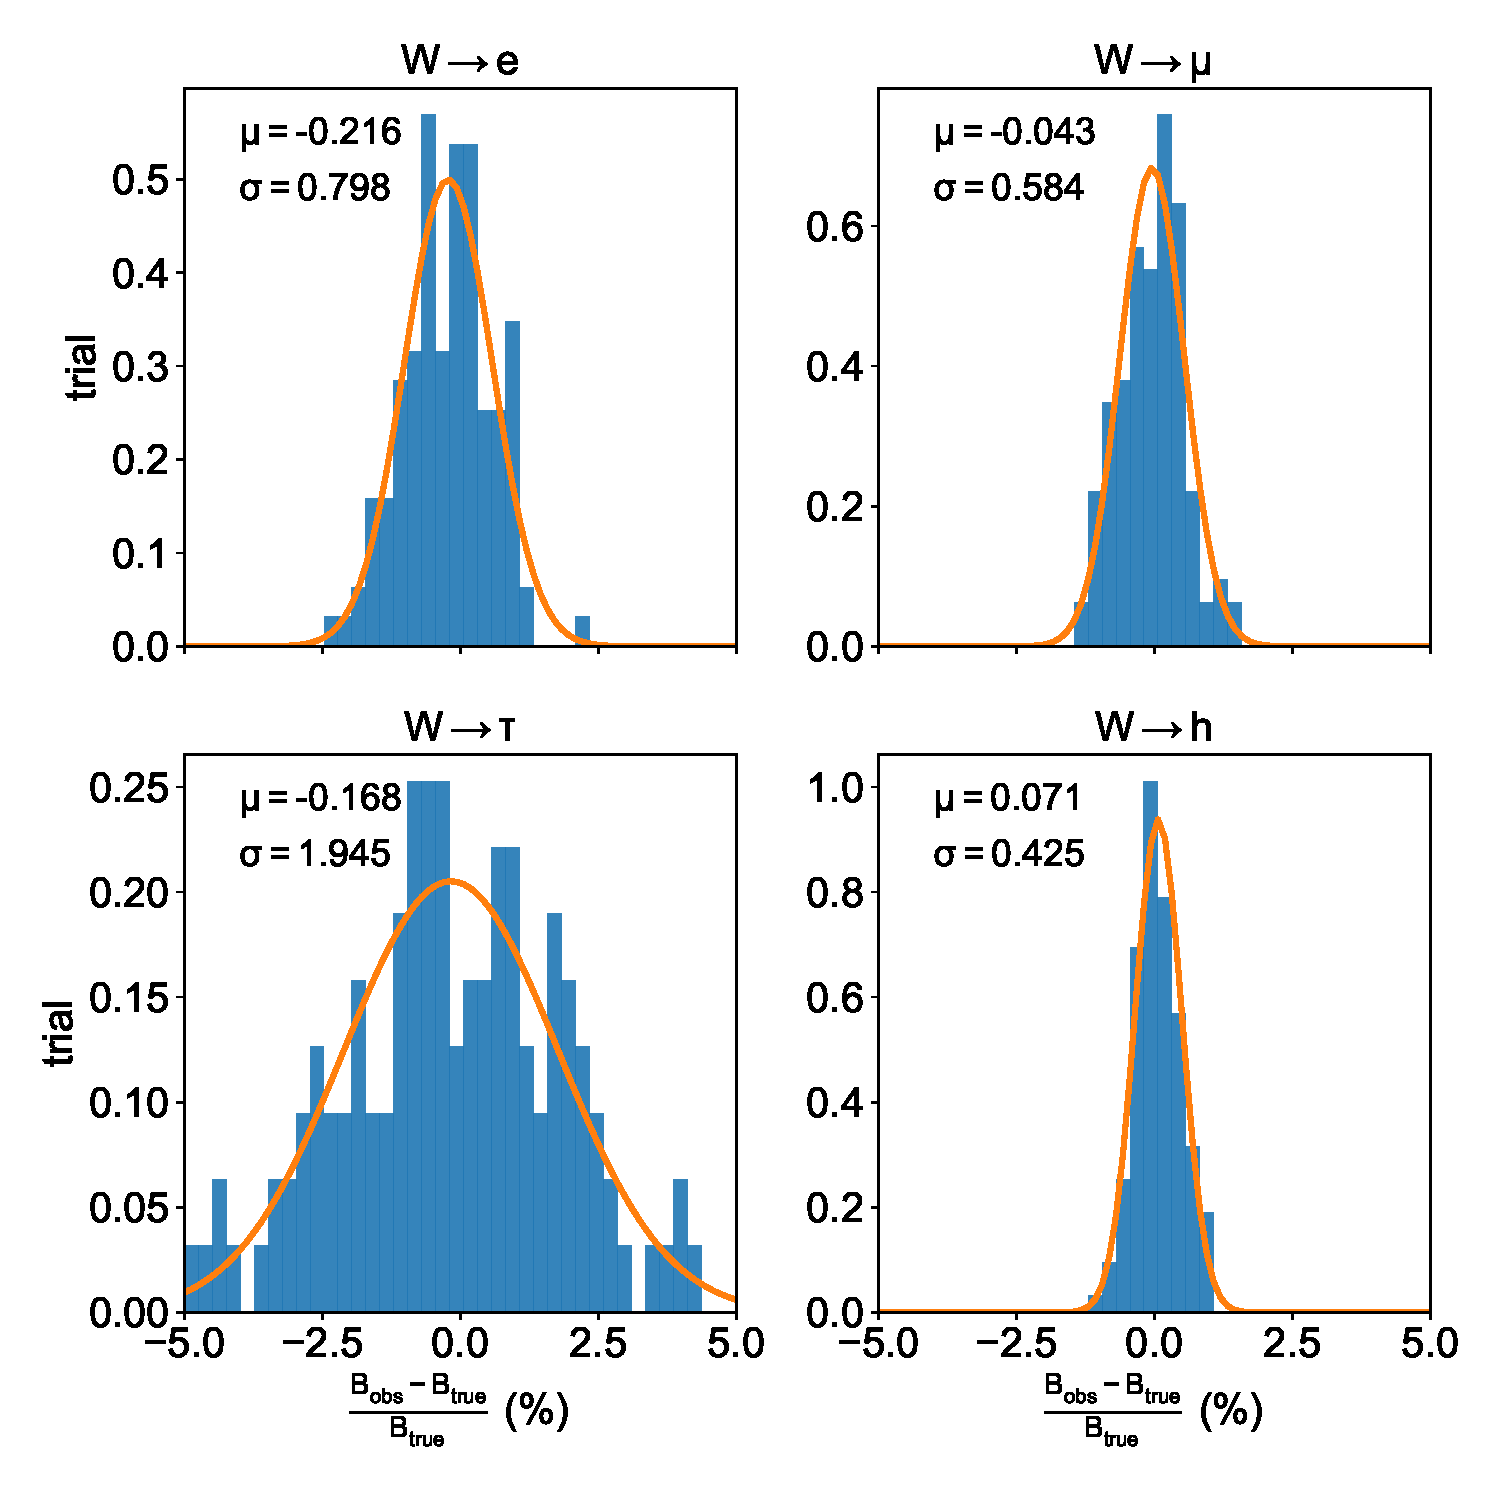
\includegraphics[width=0.7\textwidth]{chapters/Analysis/sectionStatisticalAnalysis/figures/beta_bias}
    \caption{Histogrammed values of the bias measured for each of the scan points.  The values of $\mu$ and $\sigma$ denote the mean and standard error for each distribution.}
    \label{fig:analysis:method:mle:bias_test}
\end{figure}

This study also allows for an independent estimation of the uncertainty on each of the parameters.  The resulting uncertainties estimated from the toy data are found to be close to the values calculated by carrying out a numerical estimation of the $NLL$ Hessian about its minimum.  This comparison is shown in Figure~\ref{fig:analysis:method:mle:pulls_comparison}.

\begin{sidewaysfigure}[htb!]
    \centering
    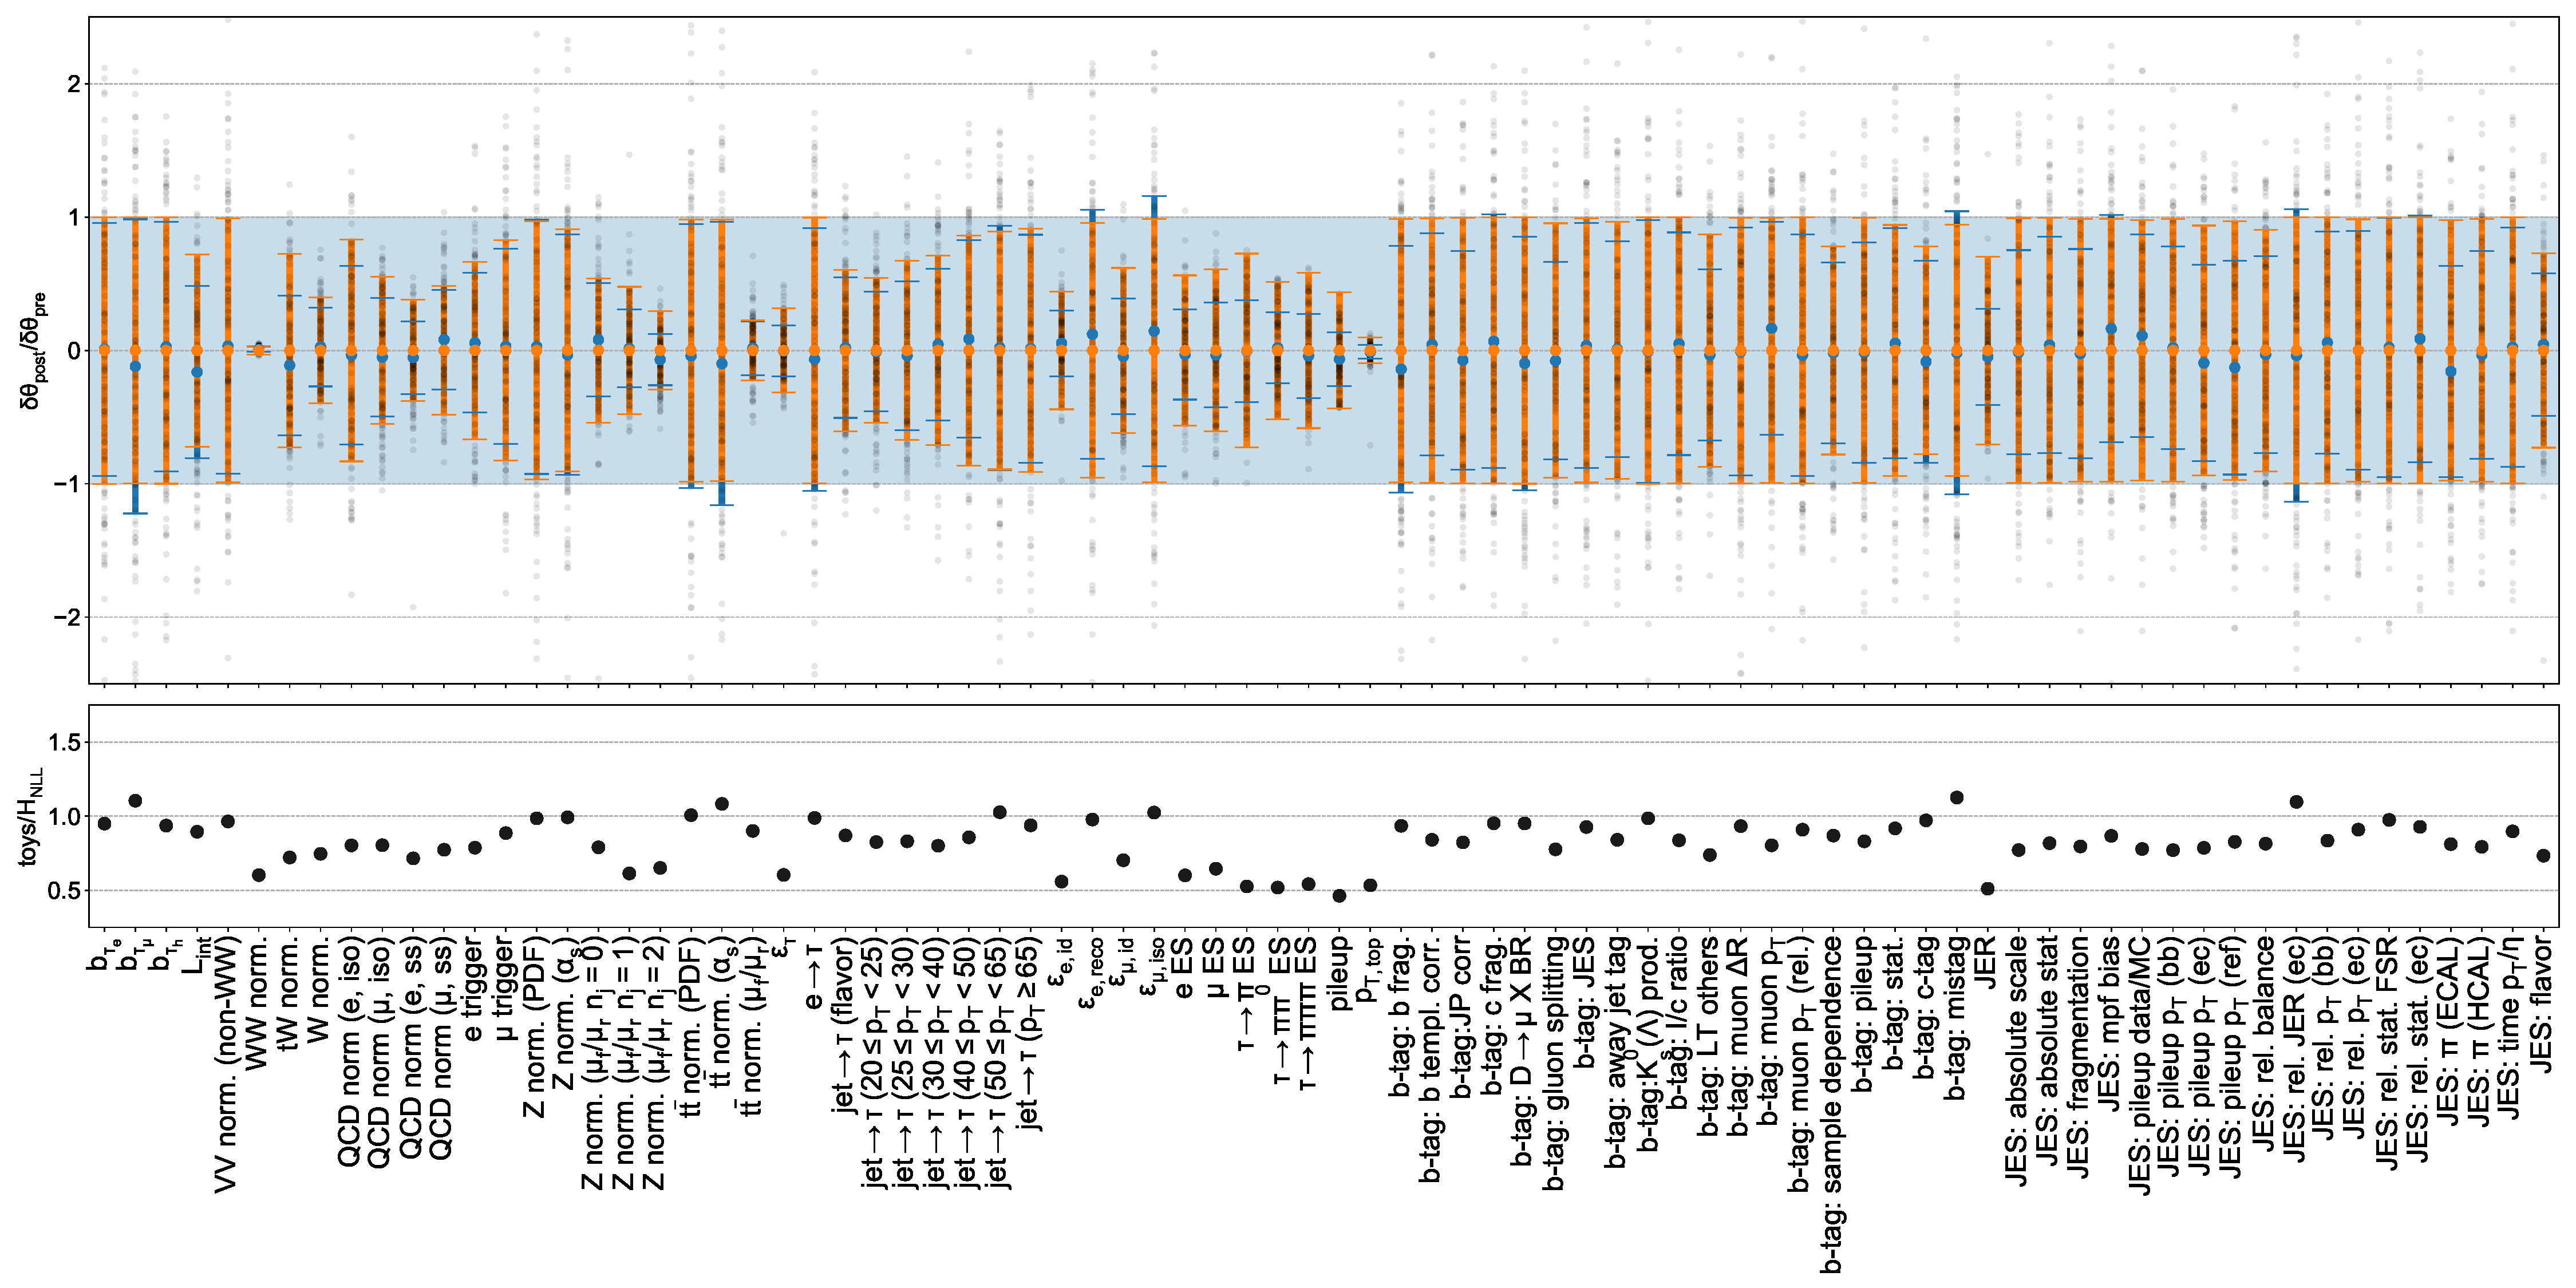
\includegraphics[width=0.9\textheight]{chapters/Analysis/sectionStatisticalAnalysis/figures/new_pulls}
    \caption{Pulls for nuisance parameters based on toy data while scanning the \PW boson leptonic branching fractions.  The black dots indicate the values for individual trials, the blue bars show the standard error estimated from those trials, and the orange bar are the values estimated from the Hessian of the negative log-likelihood $NLL$.}
    \label{fig:analysis:method:mle:pulls_comparison}
\end{sidewaysfigure}


\FloatBarrier

\subsubsection{Profile Likelihood Scans}

The covariance matrix associated with the likelihood is estimated using numerical differentiation tools~\cite{numdifftools}.  In addition to this, the variance associated with each parameter can be estimated by scanning over values of the parameter near its minimum and minimizing the likelihood while holding the parameter's value fixed.  The resulting values of the $NLL$ can then be fitted with a parabola to get the associated standard error.  Because the full likelihood is just a sum of the Poisson likelihoods for each bin, the likelihood associated with each bin can also be studied.  This is useful for analyzing which categories and which parts of the kinematical space are more sensitive to different fit parameters.  

The result of scanning over the three leptonic branching fractions is shown in figure~\ref{fig:analysis:method:mle:beta_scan_1D}.  Curvatures of the $NLL$ in each bin of the analysis are estimated in the same way and presented in figures~\ref{fig:analysis:method:mle:ele_scan_bins}, \ref{fig:analysis:method:mle:mu_scan_bins}, \ref{fig:analysis:method:mle:tau_scan_bins}. The figure shows the estimated curvature (variance) in each bin normalized to the total variance.  The simplest way to interpret what is shown is that a larger bar corresponds to a more significant contribution to the sensitivity to the parameter under consideration.

\begin{figure}[h]
    \centering
    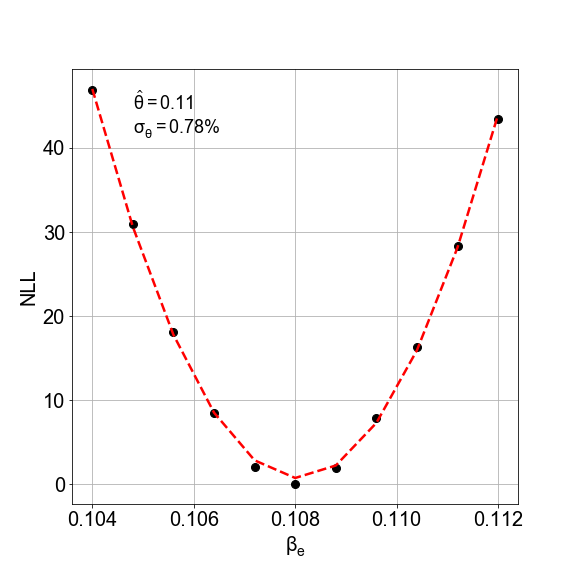
\includegraphics[width=0.32\textwidth]{chapters/Analysis/sectionStatisticalAnalysis/figures/beta_e}
    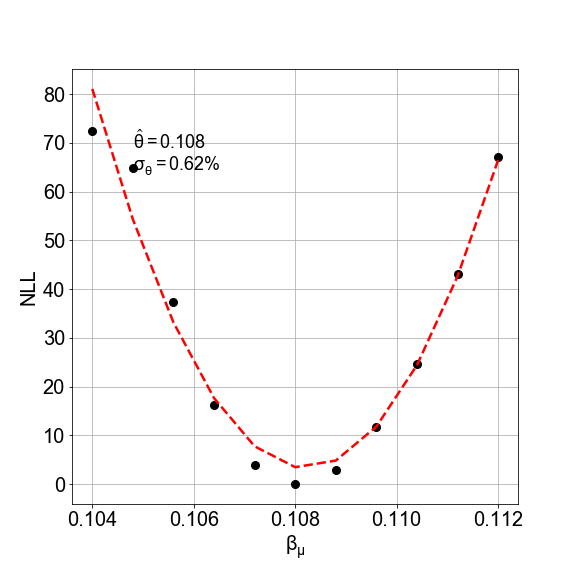
\includegraphics[width=0.32\textwidth]{chapters/Analysis/sectionStatisticalAnalysis/figures/beta_mu}
    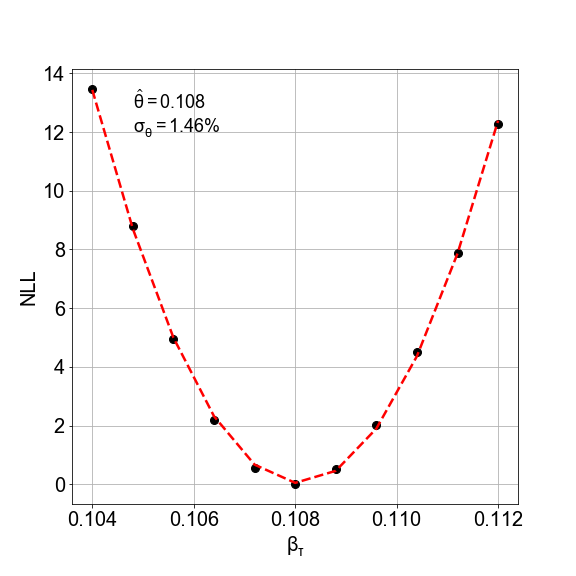
\includegraphics[width=0.32\textwidth]{chapters/Analysis/sectionStatisticalAnalysis/figures/beta_tau}
    \caption{Values for the negative log-likelihood while scanning over the leptonic branching fractions of the \PW.}
    \label{fig:analysis:method:mle:beta_scan_1D}
\end{figure}

\begin{figure}[htb!]
    \centering
    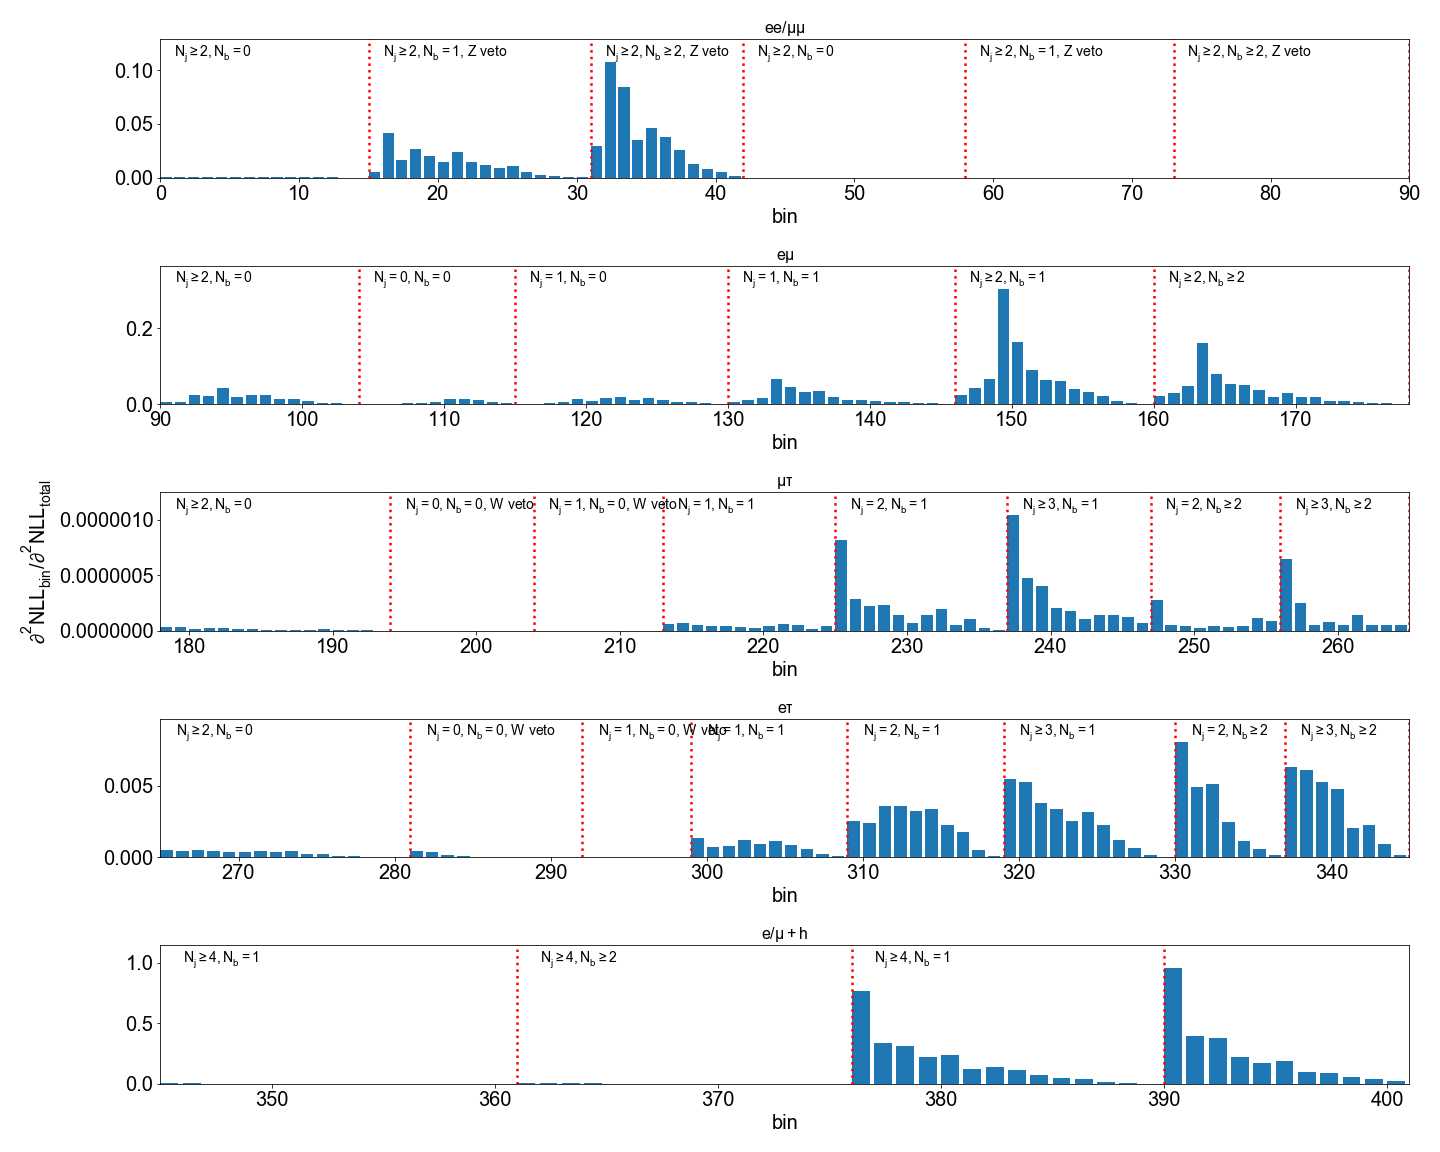
\includegraphics[width=1.2\textwidth, angle=-90]{chapters/Analysis/sectionStatisticalAnalysis/figures/beta_e_scan_bins_lh}
    \caption{Bin-by-bin sensitivity for the electronic branching fraction. }
    \label{fig:analysis:method:mle:ele_scan_bins}
\end{figure}

\begin{figure}[htb!]
    \centering
    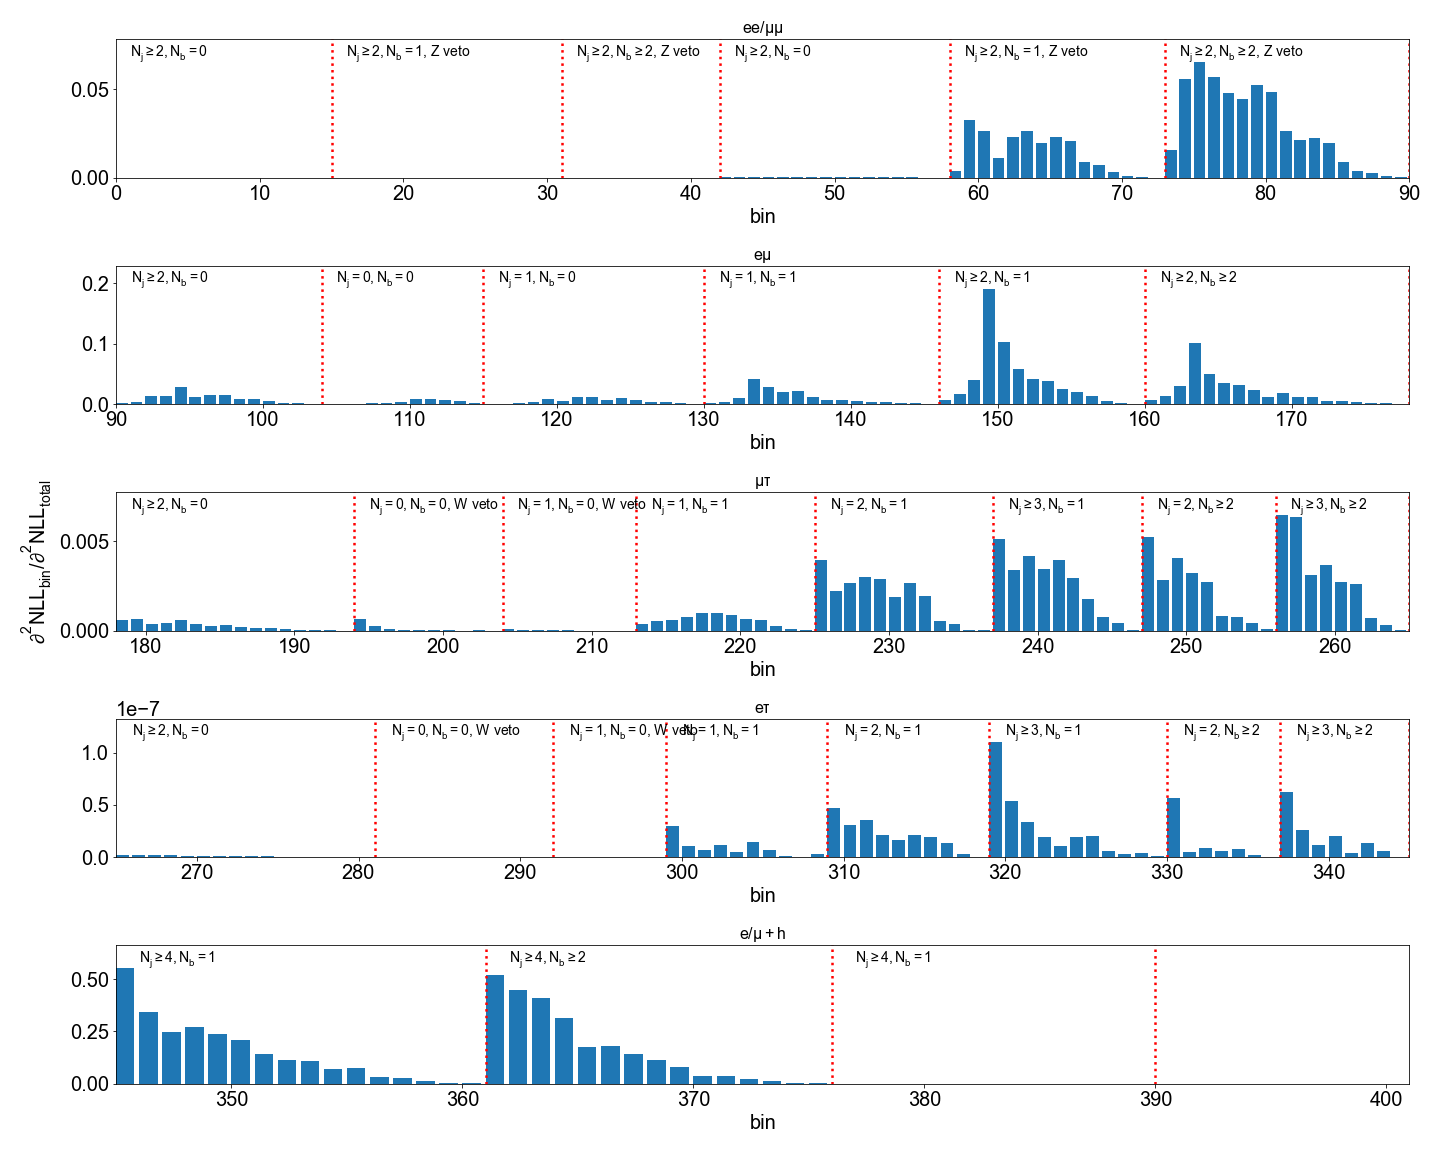
\includegraphics[width=1.2\textwidth, angle=-90]{chapters/Analysis/sectionStatisticalAnalysis/figures/beta_mu_scan_bins_lh}
    \caption{Bin-by-bin sensitivity for the muonic branching fraction.}
    \label{fig:analysis:method:mle:mu_scan_bins}
\end{figure}

\begin{figure}[htb!]
    \centering
    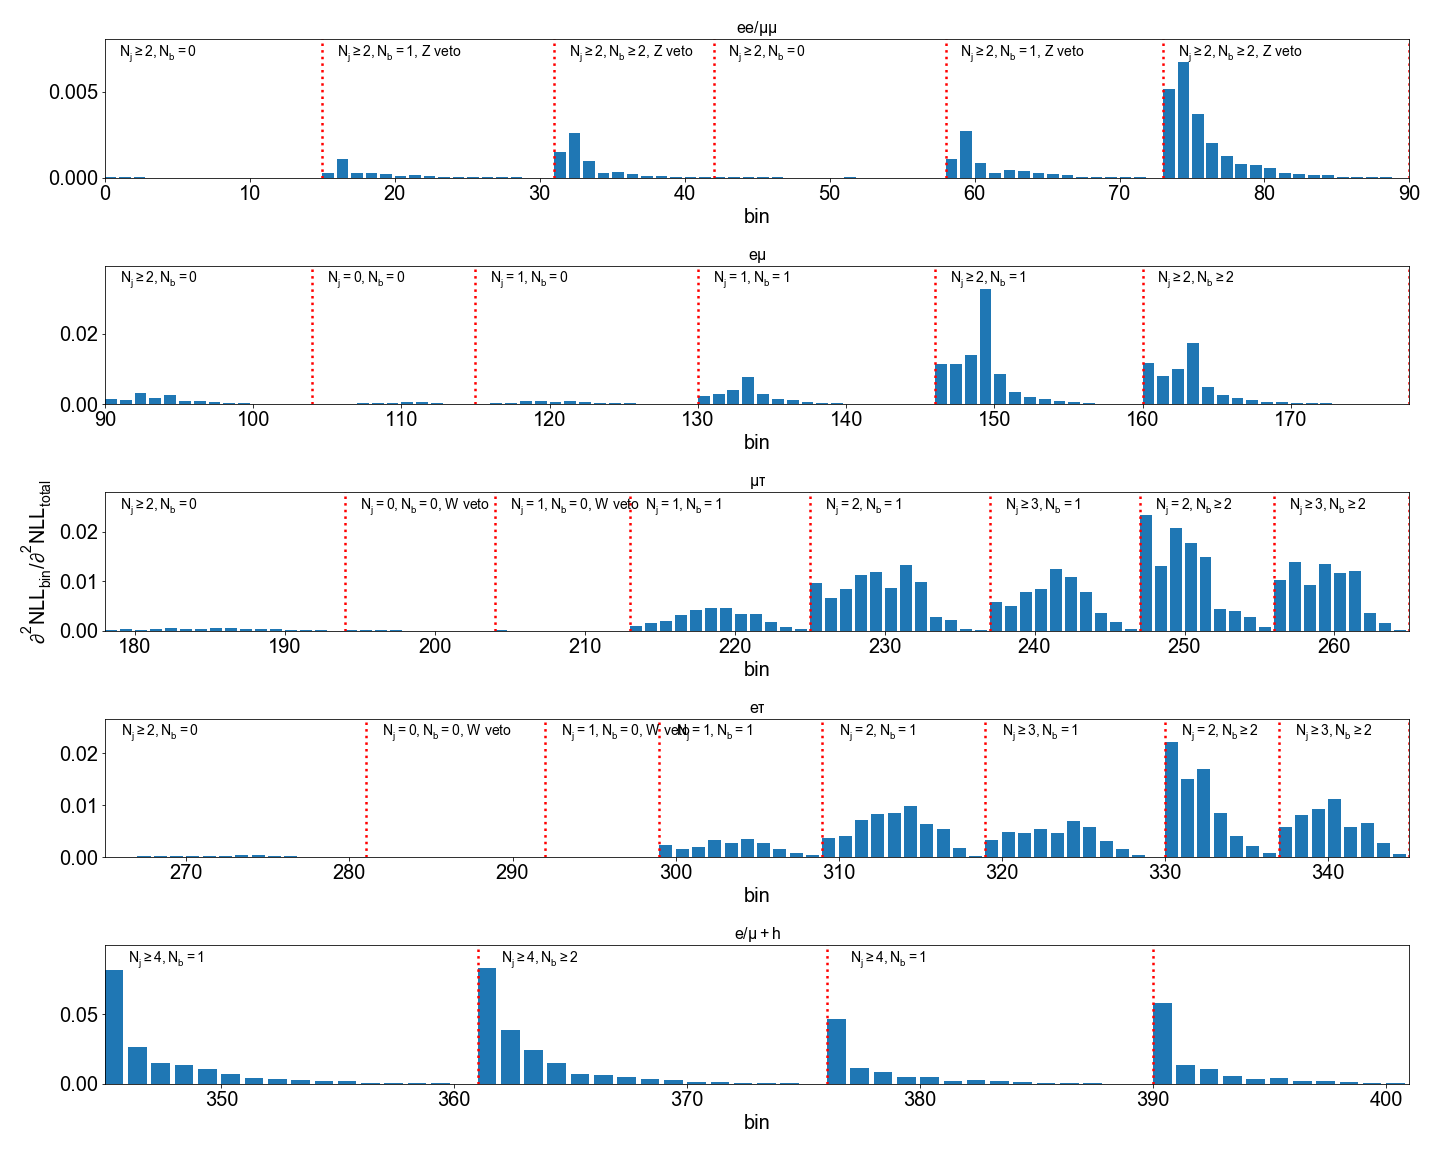
\includegraphics[width=1.2\textwidth, angle=-90]{chapters/Analysis/sectionStatisticalAnalysis/figures/beta_tau_scan_bins_lh}
    \caption{Bin-by-bin sensitivity for the tauonic branching fraction.}
    \label{fig:analysis:method:mle:tau_scan_bins}
\end{figure}


\FloatBarrier




%%%%%%%%%%%%%%%%%%%%%%%%%%%%%%%%%%%%%%%%
% 3. Counting Analysis
%%%%%%%%%%%%%%%%%%%%%%%%%%%%%%%%%%%%%%%%
\subsection{Counting Analysis}


\begin{figure}[htb!]
    \centering
    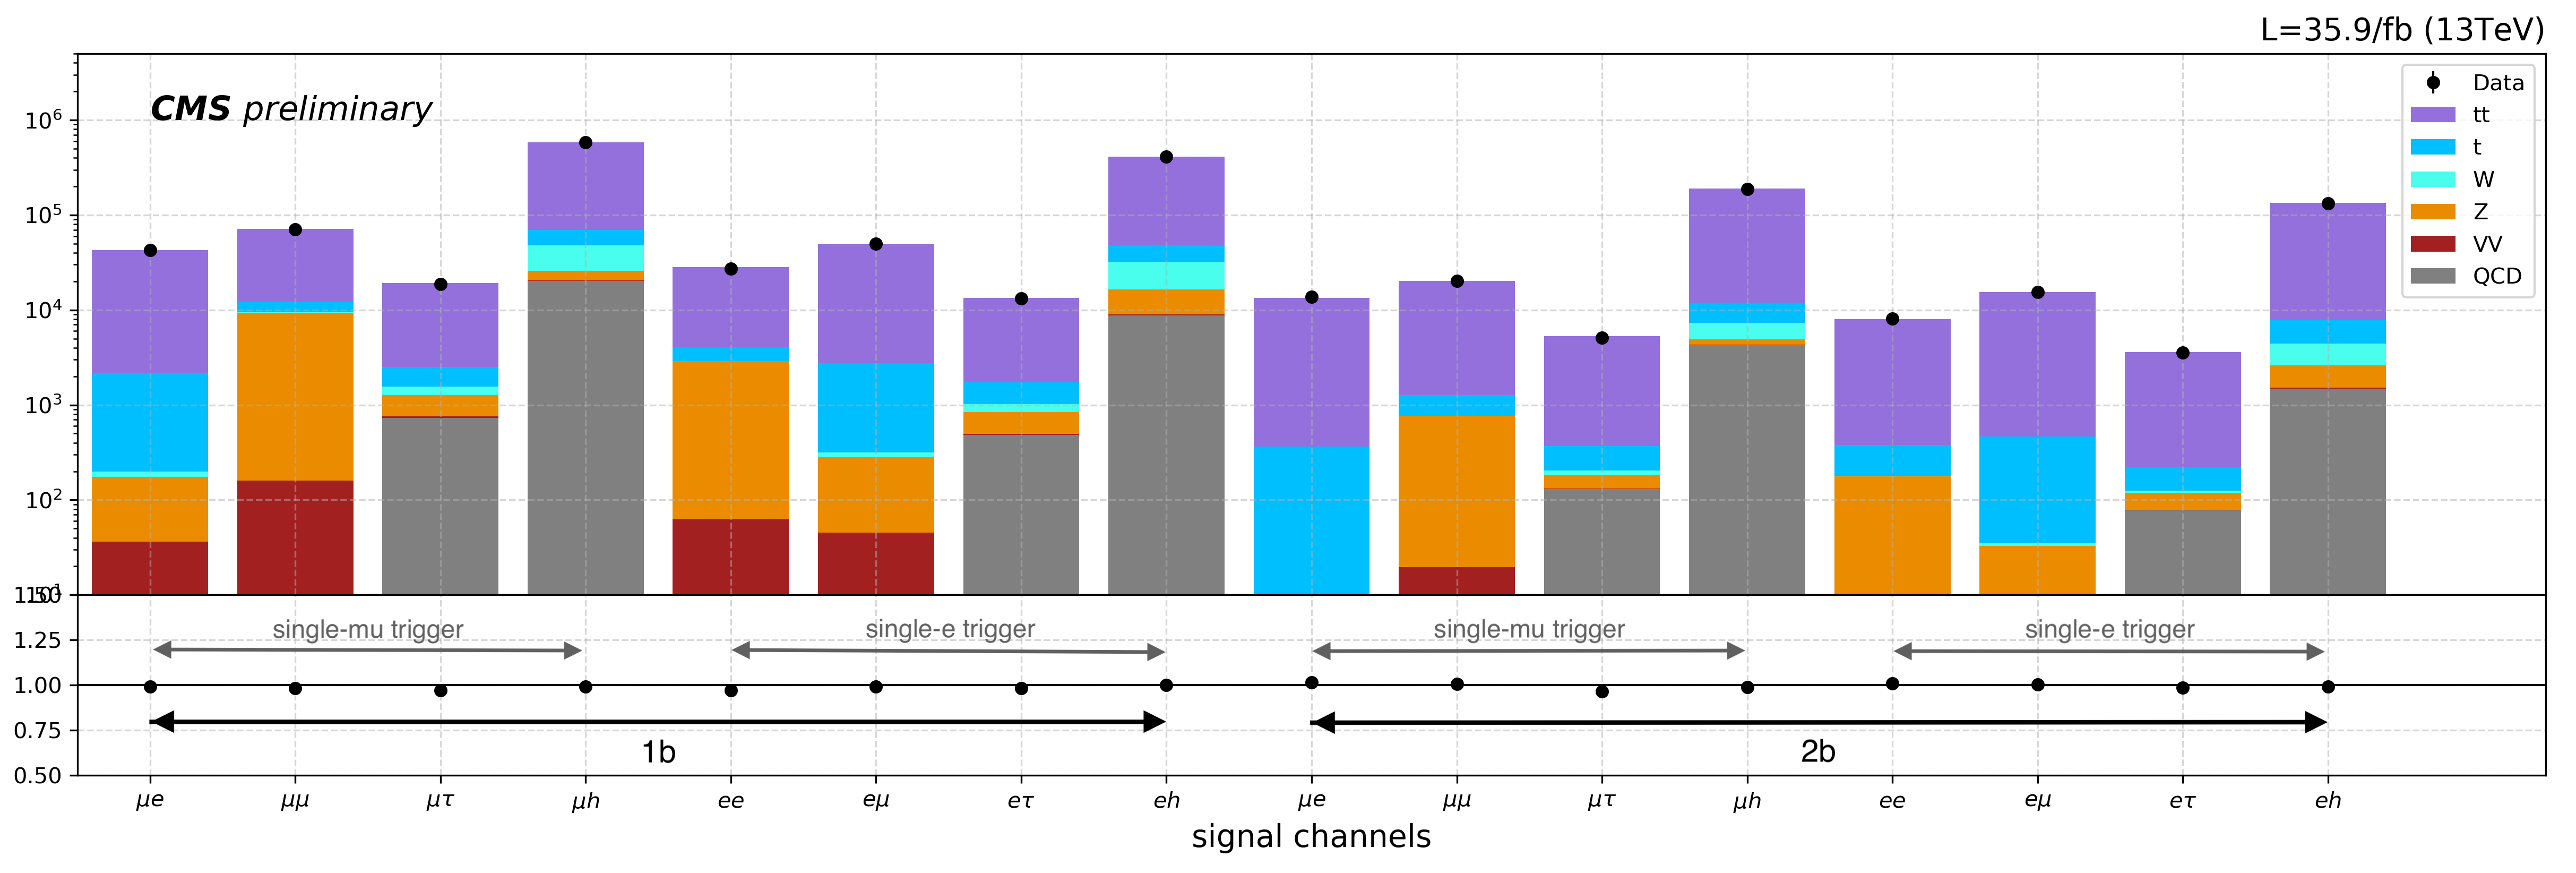
\includegraphics[width=0.99\textwidth]{chapters/Analysis/sectionStatisticalAnalysis/figures/counting.png}
    \caption{ Channels are organized into four groups based on trigger type and \PQb tag multiplicity. Counting analysis extracts \PW branching fractions from the yields of grouped channels.}
    \label{fig:analysis:method:counting:groupsofchannel}
\end{figure}

In this approach, channels are divided into four mutually-exclusive groups based on the trigger types and the \PQb tag multiplicities. The trigger types include the single-muon and the single-electron trigger. The \PQb tag multiplicity can be either $n_\PQb=1$ or $n_\PQb \geq 2$. The configuration of four channel groups is shown in figure~\ref{fig:analysis:method:counting:groupsofchannel}. Namely,

\begin{itemize}
    \item single-$\PGm$ trigger with $n_\PQb=1$ or $n_\PQb \geq 2$ : $\big \{ \PGm e, \PGm\PGm, \PGm\PGt, \PGm h \big  \}$.
    \item single-$\Pe$  trigger with $n_\PQb=1$ or $n_\PQb \geq 2$ : $ \big  \{ e e, e\PGm, e\PGt, e h \big  \}$ .
\end{itemize}


\noindent where \cem and \cme are mutually exclusive -- \cem channel requires single-$\Pe$ trigger with $\pt^\Pe > \pt^\PGm$, while \cme channel requires $\PGm$-trigger with $\pt^\Pe < \pt^\PGm$. 




To reduce contamination from $j\to \PGt$ fakes and QCD background, in the counting analysis, the thresholds of leptons' \pt  and working point for the hadronic tau isolation are slightly tighten. This results in slightly different signal efficiencies comparing with the shape analysis. For the eight channels under consideration, the signal efficiencies determined from simulated \ttbar and \tW events are shown in Tables \ref{tab:sanalysis:method:counting:igacc} and Figure~\ref{fig:analysis:method:counting:efficencyMatrix}. 

%In each of 16 channels, the signal constituents break down to 21 decay
%final states is shown in percentage in Table \ref{sigcomp}.


\begin{figure}[ht]
    \centering
    channels with $\PGm$-trigger-1b \\
    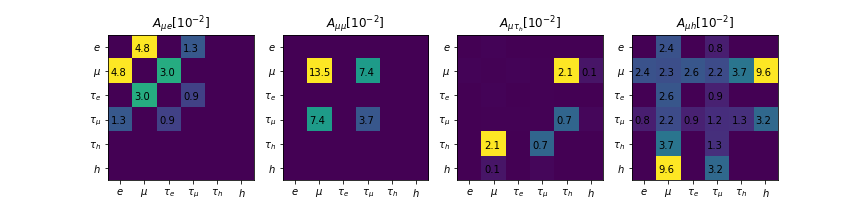
\includegraphics[width=\textwidth]{chapters/Analysis/sectionStatisticalAnalysis/figures/acc_mu1b.png}
    
    channels with $\PGm$-trigger-2b \\
    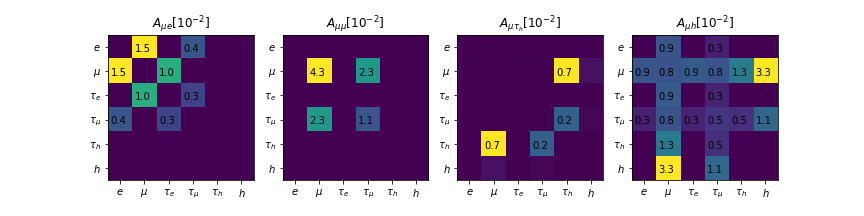
\includegraphics[width=\textwidth]{chapters/Analysis/sectionStatisticalAnalysis/figures/acc_mu2b.png}
    
    channels with $e$-trigger-1b \\
    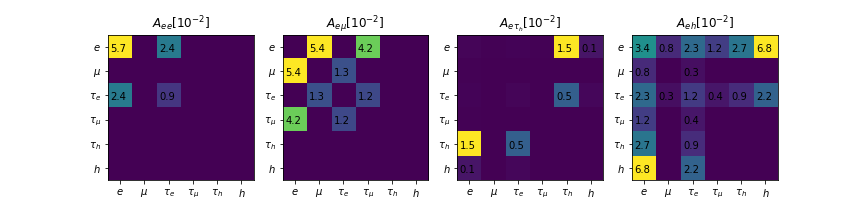
\includegraphics[width=\textwidth]{chapters/Analysis/sectionStatisticalAnalysis/figures/acc_e1b.png}
    
    channels with $e$-trigger-2b \\
    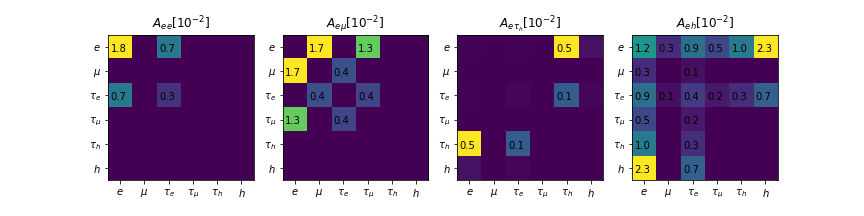
\includegraphics[width=\textwidth]{chapters/Analysis/sectionStatisticalAnalysis/figures/acc_e2b.png}
    
    %--------------------------
    \caption{ Efficiency matrices of eight channels with $n_\PQb=1$ and $n_\PQb \geq 2$. The channels are grouped based on trigger types and \PQb tag multiplicities. }
    \label{fig:analysis:method:counting:efficencyMatrix}
\end{figure}





\begin{sidewaystable}[p]
    \centering
    \setlength{\tabcolsep}{0.4em}
    \renewcommand{\arraystretch}{1.5}
    \caption{Efficiency of $t\bar{t}$+$tW$ events, breakdown by 21 WW decay.  Values are in percent.}
    
    \resizebox{\textwidth}{!}{
    \begin{tabular}{|l|cc|cc|cc|cc|cc|cc|cc|cc|}
    
    
    \hline
    channel & \multicolumn{2}{|c|}{$\mu e$} & \multicolumn{2}{c|}{$\mu\mu$} & \multicolumn{2}{|c|}{$\mu \tau$} & \multicolumn{2}{|c|}{$\mu$+jets} & \multicolumn{2}{|c|}{$ee$} & \multicolumn{2}{|c|}{$e\mu$} & \multicolumn{2}{|c|}{$e \tau$} & \multicolumn{2}{|c|}{$e+jets$} \\
    \hline
    $\rm n_{b tag}$ & $n_b=1$ & $n_b\geq2$ & $n_b=1$ & $n_b\geq2$ & $n_b=1$ & $n_b\geq2$ & $n_b=1$ & $n_b\geq2$ & $n_b=1$ & $n_b\geq2$ & $n_b=1$ & $n_b\geq2$ & $n_b=1$ & $n_b\geq2$ & $n_b=1$ & $n_b\geq2$ \\ 
    \hline
    
    $tt/tW \to ee$                     &    --    &    --    &    --    &    --    &    --    &    --    &    --    &    --    &  5.71(1) &  3.19(1) &    --    &    --    &    --    &    --    &  3.17(1) &  2.14(1) \\ 
    $tt/tW \to \mu\mu$                 &    --    &    --    & 14.14(2) &  8.02(1) &    --    &    --    &  1.80(1) &  1.21(0) &    --    &    --    &    --    &    --    &    --    &    --    &    --    &    --    \\ 
    $tt/tW \to e\mu$                   &  4.69(1) &  2.66(0) &    --    &    --    &    --    &    --    &  2.35(0) &  1.60(0) &    --    &    --    &  5.76(1) &  3.24(1) &    --    &    --    &  0.71(0) &  0.48(0) \\ 
    $tt/tW \to \tau_{e}\tau_{e}$       &    --    &    --    &    --    &    --    &    --    &    --    &    --    &    --    &  0.74(2) &  0.44(2) &    --    &    --    &    --    &    --    &  1.18(4) &  0.81(2) \\ 
    $tt/tW \to \tau_{\mu}\tau_{\mu}$   &    --    &    --    &  3.88(5) &  2.11(4) &    --    &    --    &  1.13(3) &  0.77(2) &    --    &    --    &    --    &    --    &    --    &    --    &    --    &    --    \\ 
    $tt/tW \to \tau_{e}\tau_{\mu}$     &  0.78(2) &  0.45(1) &    --    &    --    &    --    &    --    &  0.92(2) &  0.62(1) &    --    &    --    &  1.24(2) &  0.70(2) &    --    &    --    &  0.40(1) &  0.27(1) \\ 
    $tt/tW \to \tau_{e}\tau_{h}$       &    --    &    --    &    --    &    --    &    --    &    --    &    --    &    --    &    --    &    --    &    --    &    --    &  0.48(1) &  0.26(0) &  0.84(1) &  0.61(1) \\ 
    $tt/tW \to \tau_{\mu}\tau_{h}$     &    --    &    --    &    --    &    --    &  0.74(1) &  0.40(1) &  1.28(1) &  0.92(1) &    --    &    --    &    --    &    --    &    --    &    --    &    --    &    --    \\ 
    $tt/tW \to \tau_{h}\tau_{h}$       &    --    &    --    &    --    &    --    &    --    &    --    &    --    &    --    &    --    &    --    &    --    &    --    &    --    &    --    &    --    &    --    \\ 
    $tt/tW \to e\tau_{e}$              &    --    &    --    &    --    &    --    &    --    &    --    &    --    &    --    &  2.14(1) &  1.18(1) &    --    &    --    &    --    &    --    &  2.29(1) &  1.62(1) \\ 
    $tt/tW \to e\tau_{\mu}$            &  1.28(1) &  0.69(1) &    --    &    --    &    --    &    --    &  0.80(1) &  0.54(0) &    --    &    --    &  4.49(2) &  2.47(1) &    --    &    --    &  1.18(1) &  0.86(1) \\ 
    $tt/tW \to e\tau_{h}$              &    --    &    --    &    --    &    --    &    --    &    --    &    --    &    --    &    --    &    --    &    --    &    --    &  1.59(1) &  0.88(0) &  2.61(1) &  1.90(0) \\ 
    $tt/tW \to \mu\tau_{e}$            &  2.54(1) &  1.43(1) &    --    &    --    &    --    &    --    &  2.61(1) &  1.86(1) &    --    &    --    &  1.42(1) &  0.78(1) &    --    &    --    &  0.23(0) &  0.16(0) \\ 
    $tt/tW \to \mu\tau_{\mu}$          &    --    &    --    &  7.76(2) &  4.37(2) &    --    &    --    &  1.88(1) &  1.35(1) &    --    &    --    &    --    &    --    &    --    &    --    &    --    &    --    \\ 
    $tt/tW \to \mu\tau_{h}$            &    --    &    --    &    --    &    --    &  2.27(1) &  1.27(0) &  3.70(1) &  2.70(1) &    --    &    --    &    --    &    --    &    --    &    --    &    --    &    --    \\ 
    $tt/tW \to eh$                     &    --    &    --    &    --    &    --    &    --    &    --    &    --    &    --    &    --    &    --    &    --    &    --    &  0.10(0) &    --    &  6.83(0) &  4.64(0) \\ 
    $tt/tW \to \mu h$                  &    --    &    --    &    --    &    --    &  0.15(0) &    --    &  9.71(1) &  6.61(0) &    --    &    --    &    --    &    --    &    --    &    --    &    --    &    --    \\ 
    $tt/tW \to \tau_{e}h$              &    --    &    --    &    --    &    --    &    --    &    --    &    --    &    --    &    --    &    --    &    --    &    --    &    --    &    --    &  2.17(1) &  1.44(0) \\ 
    $tt/tW \to \tau_{\mu}h$            &    --    &    --    &    --    &    --    &    --    &    --    &  3.30(1) &  2.19(1) &    --    &    --    &    --    &    --    &    --    &    --    &    --    &    --    \\ 
    $tt/tW \to \tau_{h}h$              &    --    &    --    &    --    &    --    &    --    &    --    &    --    &    --    &    --    &    --    &    --    &    --    &    --    &    --    &    --    &    --    \\ 
    $tt/tW \to hh$                     &    --    &    --    &    --    &    --    &    --    &    --    &    --    &    --    &    --    &    --    &    --    &    --    &    --    &    --    &    --    &    --    \\ 

    \hline
    \end{tabular}}
    
    \label{tab:sigacc}
    
\end{sidewaystable}





\subsubsection{Parameter Extraction}


In each of the groups above, three branching fractions $\bwe,\bwm,\bwt$ are extracted by solving a set of three quadratic equations. Then the results from all four groups are combined taking into account the uncorrelated statistical uncertainties and full-correlated systematic uncertainties. The details of the combine is described in Section~\ref{sec:analysis:systematics}. Here gives the method of parameter extraction by establishing and solving quadratic equations.


The normalized yield $X$, which is constructed in a similar manner to the branching fractions, is the ratio of yield in one channel over the sum of yields in the channel group. For channel group using single-electron and single-muon trigger, denoting the triggering lepton as $\mathrm{t} \in \{\PGm, \Pe\}$, the normalized yields $X$'s are defined as
\begin{equation}
    X_\Pe   = \frac{n^{\ctre}  }{n^{\ctre} + n^{\ctrm} + n^{\ctrt} + n^{\ctrh}},
    X_\PGm  = \frac{n^{\ctrm}  }{n^{\ctre} + n^{\ctrm} + n^{\ctrt} + n^{\ctrh}}, 
    X_\PGt  = \frac{n^{\ctrt}  }{n^{\ctre} + n^{\ctrm} + n^{\ctrt} + n^{\ctrh}},
\end{equation}

\noindent where $n \equiv N - \sum_{b} N_b $ is the data yield with background subtracted. Based on Eqn \ref{eqn:analysis:method:effMatrix:data_model}, the normalized yields $\{X_\Pe,X_\PGm,X_\PGt\}$ from data should equal to the same calculation based on the efficiency $\boldsymbol{E}$ matrix and the branching fraction matrix $\boldsymbol{B}$:
% 
\begin{equation} \label{eqn:analysis:method:counting:quadEqA}
    \begin{split}
    X_e     &= \frac{ \Eij^{\ctre}\Bij }{  \Eij^{\ctre}\Bij+ \Eij^{\ctrm}\Bij+ \Eij^{\ctrt}\Bij+ \Eij^{\ctrh}\Bij} ,\\
    X_\PGm  &= \frac{ \Eij^{\ctrm}\Bij }{  \Eij^{\ctre}\Bij+ \Eij^{\ctrm}\Bij+ \Eij^{\ctrt}\Bij+ \Eij^{\ctrh}\Bij} ,\\
    X_\PGt  &= \frac{ \Eij^{\ctrt}\Bij }{  \Eij^{\ctre}\Bij+ \Eij^{\ctrm}\Bij+ \Eij^{\ctrt}\Bij+ \Eij^{\ctrh}\Bij}.
    \end{split}
\end{equation}


\noindent Plugging in the explicit form of $\boldsymbol{E}$ and $\boldsymbol{B}$ matrices in Equation~\ref{eqn:analysis:method:effMatrix:br_matrix} and \ref{eqn:analysis:method:effMatrix:eff_matrix} and the unitarity condition $\bwh=1-\bwe-\bwm-\bwt$, Equation~\ref{eqn:analysis:method:counting:quadEqA} can be written as a set of
three quadratic equations with three unknowns $\{\bwe,\bwm,\bwt\}$.
% 
% \begin{singlespace}
\begin{equation} \label{eqn:analysis:method:counting:quadEqB}
	\begin{split}
        F_e(\bwe,\bwm,\bwt) = c_{\Pe1} \bwe^2 + c_{\Pe2} \bwm^2 + c_{\Pe3} \bwt^2 + c_{\Pe4} \bwe\bwm + c_{\Pe5} \bwe\bwt + c_{\Pe6} \bwm\bwt &\\
        + c_{\Pe7} \bwe + c_{\Pe8} \bwm + c_{\Pe9} \bwt + c_{\Pe0} &= 0 ,\\
        %
        F_\PGm(\bwe,\bwm,\bwt) = c_{\PGm 1} \bwe^2 + c_{\PGm 2} \bwm^2 + c_{\PGm 3} \bwt^2 + c_{\PGm 4} \bwe\bwm + c_{\PGm 5} \bwe\bwt + c_{\PGm 6} \bwm\bwt &\\
        + c_{\PGm 7} \bwe + c_{\PGm 8} \bwm + c_{\PGm 9} \bwt + c_{\PGm 0} &= 0 , \\
        %
        F_\PGt(\bwe,\bwm,\bwt) = c_{_\PGt1} \bwe^2 + c_{\PGt2} \bwm^2 + c_{\PGt3} \bwt^2 + c_{\PGt4} \bwe\bwm + c_{\PGt5} \bwe\bwt + c_{\PGt6} \bwm\bwt &\\
        + c_{\PGt7} \bwe + c_{\PGt8} \bwm + c_{\PGt9} \bwt + c_{\PGt0} &= 0 , \\
    \end{split}
\end{equation}
% \end{singlespace}


\noindent where the coefficients $c_{lk}$, with the index $l\in \{ \Pe,\PGm,\PGt \}$ corresponding to the three equations $F_\Pe=0,F_\PGm=0,F_\PGt=0$ and the index $k\in\{ 0,1,2,\dots 9\}$, are fully determined by efficiency matrix $\boldsymbol{E}$ and normalized yields $\{X_e,X_\PGm,X_\PGt\}$. The analytical result of $c_{lk}$ is listed in table~\ref{tab:analysis:method:counting:quadcoeff}.

\begin{table}[ht]
    \centering
   	\setlength{\tabcolsep}{0.4em}
    \renewcommand{\arraystretch}{1.5}
    \small
    
    \begin{tabular}{c|l}

    \hline
    $c_{l0}$ & $\Delta_{hh}$ \\
    \hline
    $c_{l1}$ & $\Delta_{ee}     - 2\Delta_{eh}   + \Delta_{hh}$ \\
    \hline
    $c_{l2}$ & $\Delta_{\mu\mu} - 2\Delta_{\mu h} + \Delta_{hh}$ \\
    \hline
    
    $c_{l3}$ & $   b^\tau_e   b^\tau_e   \Delta_{\tau_e   \tau_e}  
    			 + b^\tau_\mu b^\tau_\mu \Delta_{\tau_\mu \tau_\mu}
                 + b^\tau_h   b^\tau_h   \Delta_{\tau_h   \tau_h}
                 
                 + 2 b^\tau_e   b^\tau_\mu \Delta_{\tau_e   \tau_\mu} 
    		     + 2 b^\tau_e   b^\tau_h   \Delta_{\tau_e   \tau_h}   
    		     + 2 b^\tau_\mu b^\tau_h   \Delta_{\tau_\mu \tau_h} - $ \\
                 
             & $   2 b^\tau_e   \Delta_{e   \tau_h}
                 - 2 b^\tau_\mu \Delta_{\mu \tau_h}
                 - 2 b^\tau_h   \Delta_{h.  \tau_h} 
                 + \Delta_{hh} $ \\

    \hline
    $c_{l4}$ & $2\Delta_{e\mu} - 2\Delta_{eh} -2\Delta_{\mu h} +2\Delta_{hh}$  \\
    \hline
    $c_{l5}$ & $  2b^\tau_e   \Delta_{e \tau_e} 
    			+ 2b^\tau_\mu \Delta_{e \tau_\mu}
                + 2b^\tau_h   \Delta_{e \tau_h}
                - 2b^\tau_e   \Delta_{\tau_e   h} 
    			- 2b^\tau_\mu \Delta_{\tau_\mu h}
                - 2b^\tau_h   \Delta_{\tau_h   h} 
                - 2\Delta_{eh}   + 2 \Delta_{hh} $ \\
        
    \hline            
    $c_{l6}$ & $  2b^\tau_e   \Delta_{\mu \tau_e} 
    			+ 2b^\tau_\mu \Delta_{\mu \tau_\mu}
                + 2b^\tau_h   \Delta_{\mu \tau_h}
                - 2b^\tau_e   \Delta_{\tau_e   h} 
    			- 2b^\tau_\mu \Delta_{\tau_\mu h}
                - 2b^\tau_h   \Delta_{\tau_h   h} 
                - 2\Delta_{\mu h}   + 2 \Delta_{hh} $ \\
    \hline            
    $c_{l7}$ & $ 2\Delta_{eh}      - 2 \Delta_{hh} $ \\
    \hline
    $c_{l8}$ & $ 2\Delta_{\mu h}   - 2 \Delta_{hh}$ \\
    \hline
    $c_{l9}$ & $  2b^\tau_e   \Delta_{\tau_e   h} 
                 + 2b^\tau_\mu \Delta_{\tau_\mu h} 
                 + 2b^\tau_h   \Delta_{\tau_h   h} 
                 - 2 \Delta_{hh}$ \\
    \hline
    \hline
    where  & $ \Delta \equiv E^{tl} - X_l \times ( E^{te} + E^{t\mu} + E^{t\tau} + E^{th} )$ \\
           & $l=e,\mu,\tau$ and $t=e(\mu)$ if using single-$e$ (signle-$\mu$) trigger\\
    \hline
    
	\end{tabular}
    
\caption{ Coefficients of quadratic equations in terms of E and X. In the table, $l=e,\mu,\tau$ and $t=\mu,e$ for single-$\mu$ and single-$e$ trigger respectively.  }
\label{quadcoeff}
    
\end{table}

\begin{figure}[ht]
    \centering
    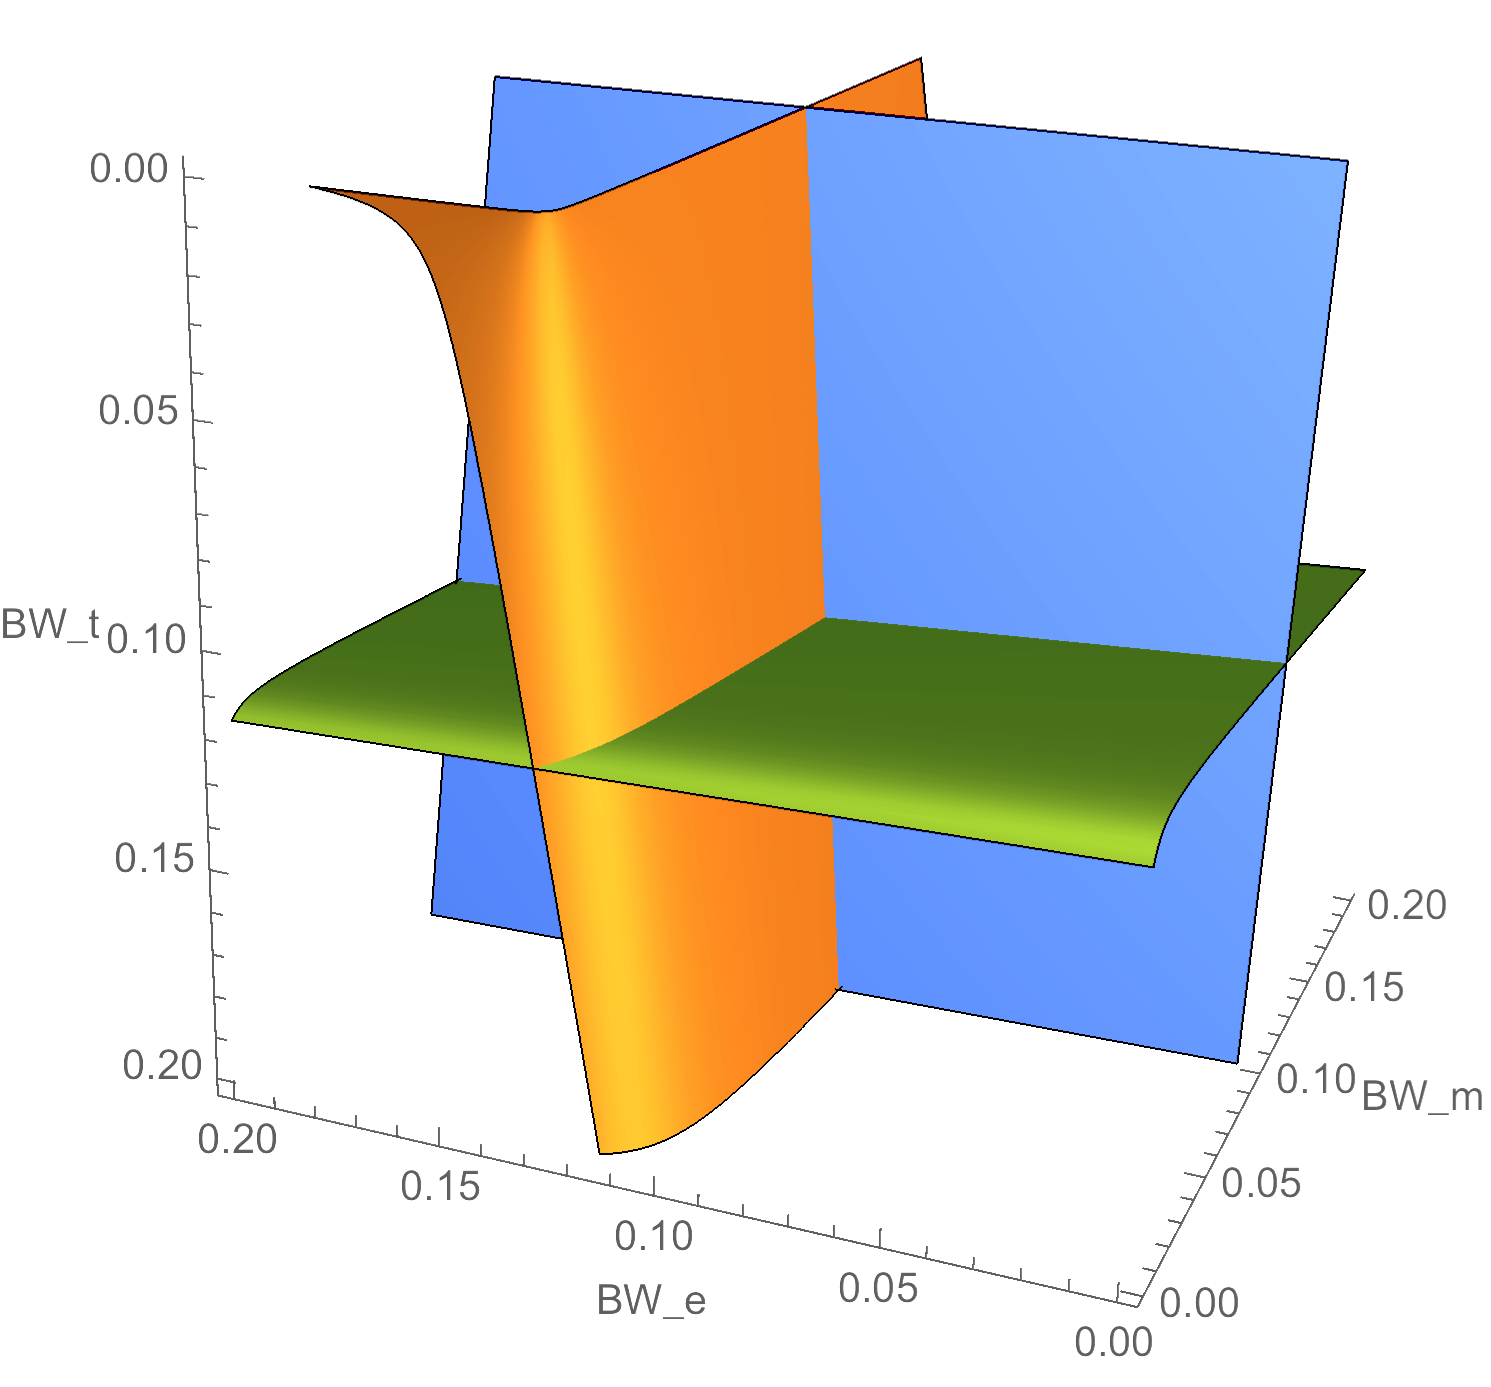
\includegraphics[width=7cm]{chapters/Analysis/sectionStatisticalAnalysis/figures/visual.png}
    \caption{ Visualization of Equation~\ref{eqn:analysis:method:counting:quadEqB} in the $\{\bwe,\bwm,\bwt\}$ parameter space. Each equation is a hyperbolic plane, while their
    intersection is the solution. Mathematically, there are 8 possible solutions. However, only one solution is physical, located with $\beta \in (0,1) $. }
    \label{fig:analysis:method:counting:visualize}
\end{figure}


In the $\{\bwe,\bwm,\bwt\}$ parameter space, Equation~\ref{eqn:analysis:method:counting:quadEqB} represents three hyperbolic planes. Figure~\ref{fig:analysis:method:counting:visualize} shows a visualization of the three hyperbolic planes in the $\{\bwe,\bwm,\bwt\}$ parameter space. The intersection of the three planes is the solution to the three quardatic equations, which presents the measurement of branching fractions. Namely,
% 
\begin{equation} 
    \begin{bmatrix} \bwe \\ \bwm \\ \bwt \end{bmatrix} = \text{Solution}
    \begin{bmatrix}
	    F_e    (\bwe,\bwm,\bwt)  = 0 \\
	    F_\PGm  (\bwe,\bwm,\bwt) = 0 \\
	    F_\PGt (\bwe,\bwm,\bwt)  = 0
    \end{bmatrix}
\end{equation}



\subsubsection{Assessment of Statistical Uncertainties}
The statistical uncertainties of data are propagated to the branching fraction via the numerically calculated partial derivatives $\partial_{N} \beta$. The statistical uncertainties of yields in different channels are treated as uncorrelated, and are summed in quadrature after being propagated to $\beta$.

The statistical uncertainties due to the simulation are estimated by the same error propagation approach. For \ttbar and \tW simulation, the statistical uncertainties are embedded in the statistical uncertainties of the $E$ matrix based on equation~\ref{eqn:analysis:method:effMatrix:model_eff}. The statistical uncertainty of efficiency, obtained by an integral of beta distribution, the conjugate of the binomial distribution, is propagated to the $\beta$ the partial derivatives $\partial_{\epsilon} \beta$. The 21 efficiencies in the $E$ matrix are treated as uncorrelated and their impacts to $\beta$ are summed in quadrature. For other background simulation, the statistical uncertainties is propagated to $\beta$ via partial derivatives $\partial_{N_{\rm bkg}} \beta$ similar to that of data.


\subsubsection{Assessment of Systematic Uncertainties}

The systematic uncertainties are estimated by variating up and down the systematic parameters, and then repeating the same process of parameter extraction. The corresponding deviations with respect to the nominal $\beta$ represent the systematic uncertainties. Different systematic sources are treated as independent. The systematic uncertainties in different trigger-$n_\PQb$ groups are fully-correlated.


\subsubsection{Bias Study of Parameter Extraction}
A test of parameter extraction is performed using toy datasets. In toy datasets, the yield $N$ follow the normal distribution with a mean value equals to the expected yield based on simulated datasets and QCD estimation, and a standard deviation equals $\delta N = \sqrt{N}$. Then $\beta$ are extracted from each toy dataset. In total, two thousand toy datasets are generated. The \PW to lepton branching fractions in the simulation is $10.8\%$, which is the ground truth to compare the extracted parameters. The distribution of two thousand $\{\bwe,\bwm,\bwt\}$ extracted are shown in Figure~\ref{fig:analysis:method:counting:test_toy}. The centers of distributions are consistent with the assumed branching fraction in the simulation, while widths of distributions are consistent with the data statistical uncertainty calculated by error propagation.





\begin{figure}[ht]
    \centering
    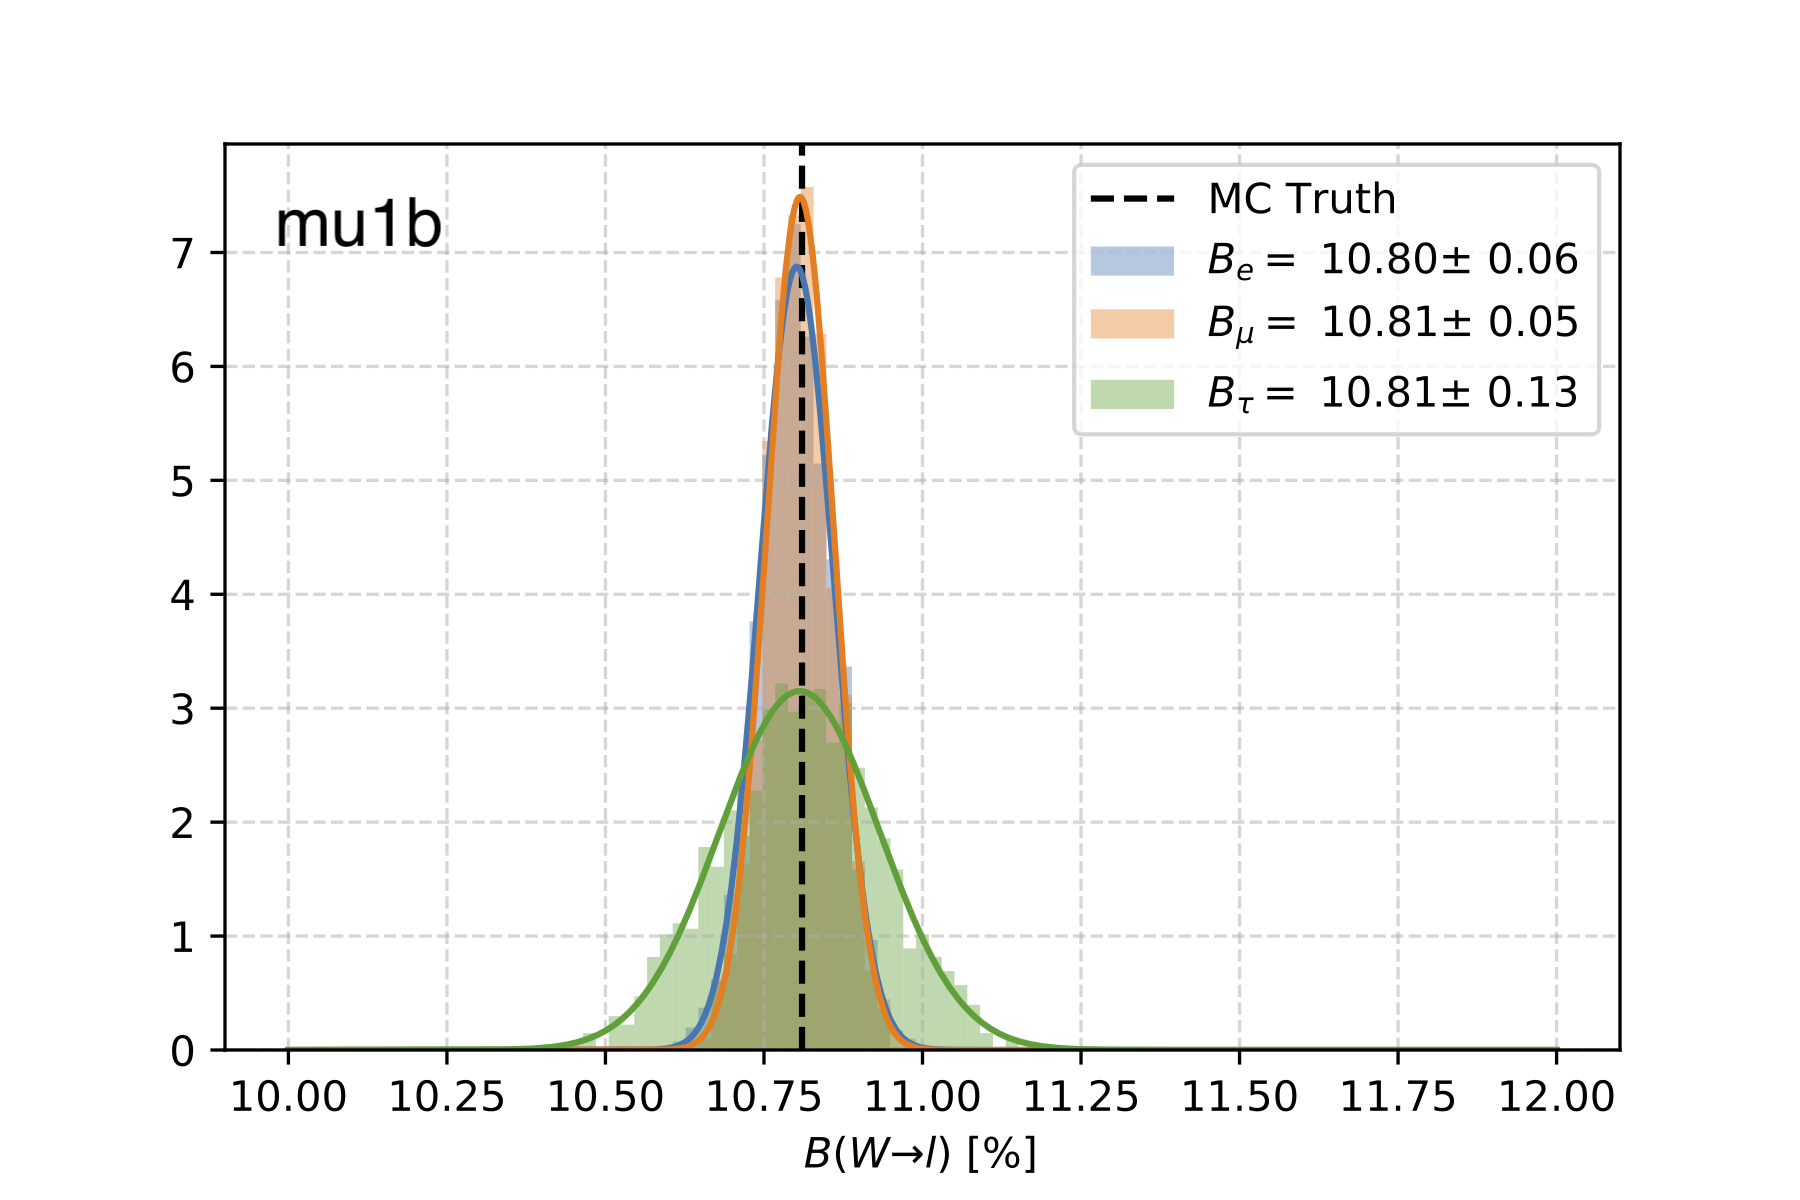
\includegraphics[width=7cm]{chapters/Analysis/sectionStatisticalAnalysis/figures/test_mu1b.png}
    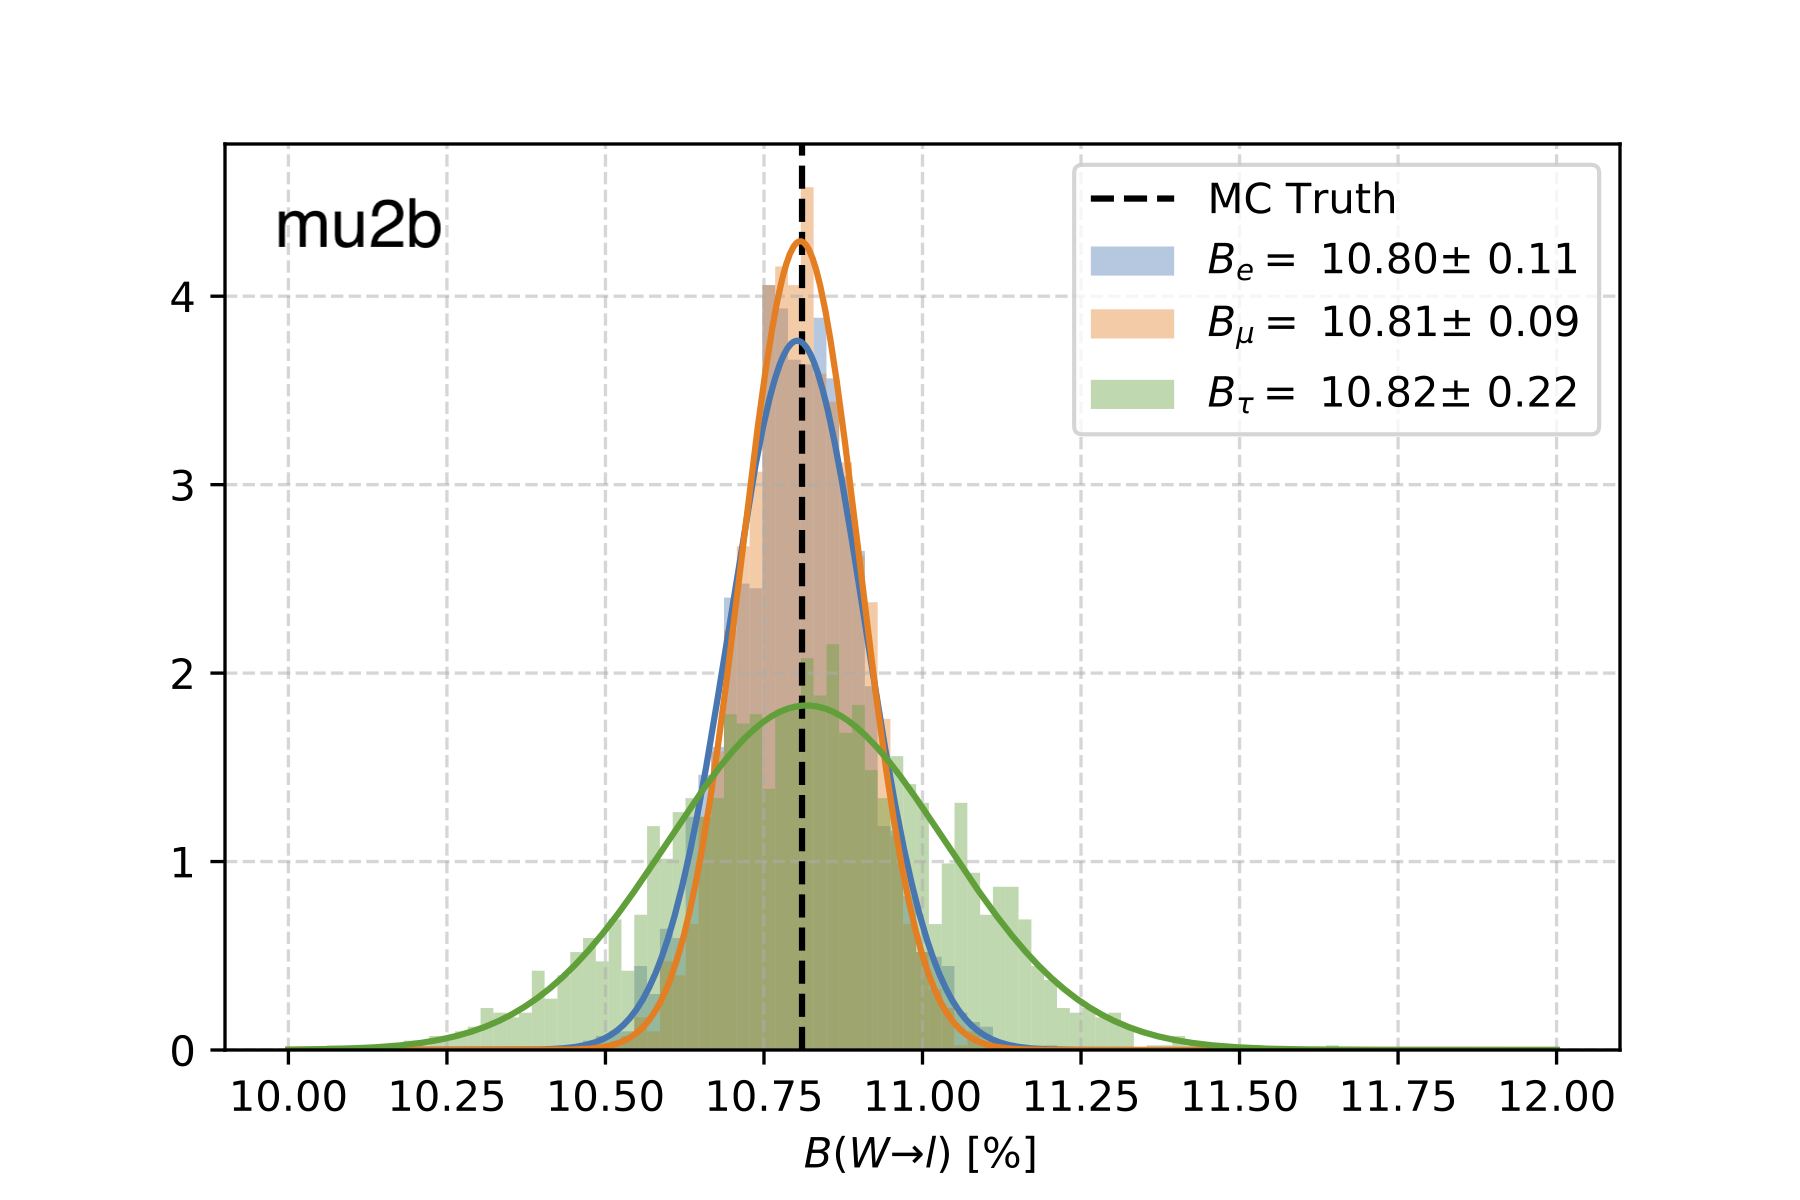
\includegraphics[width=7cm]{chapters/Analysis/sectionStatisticalAnalysis/figures/test_mu2b.png}
    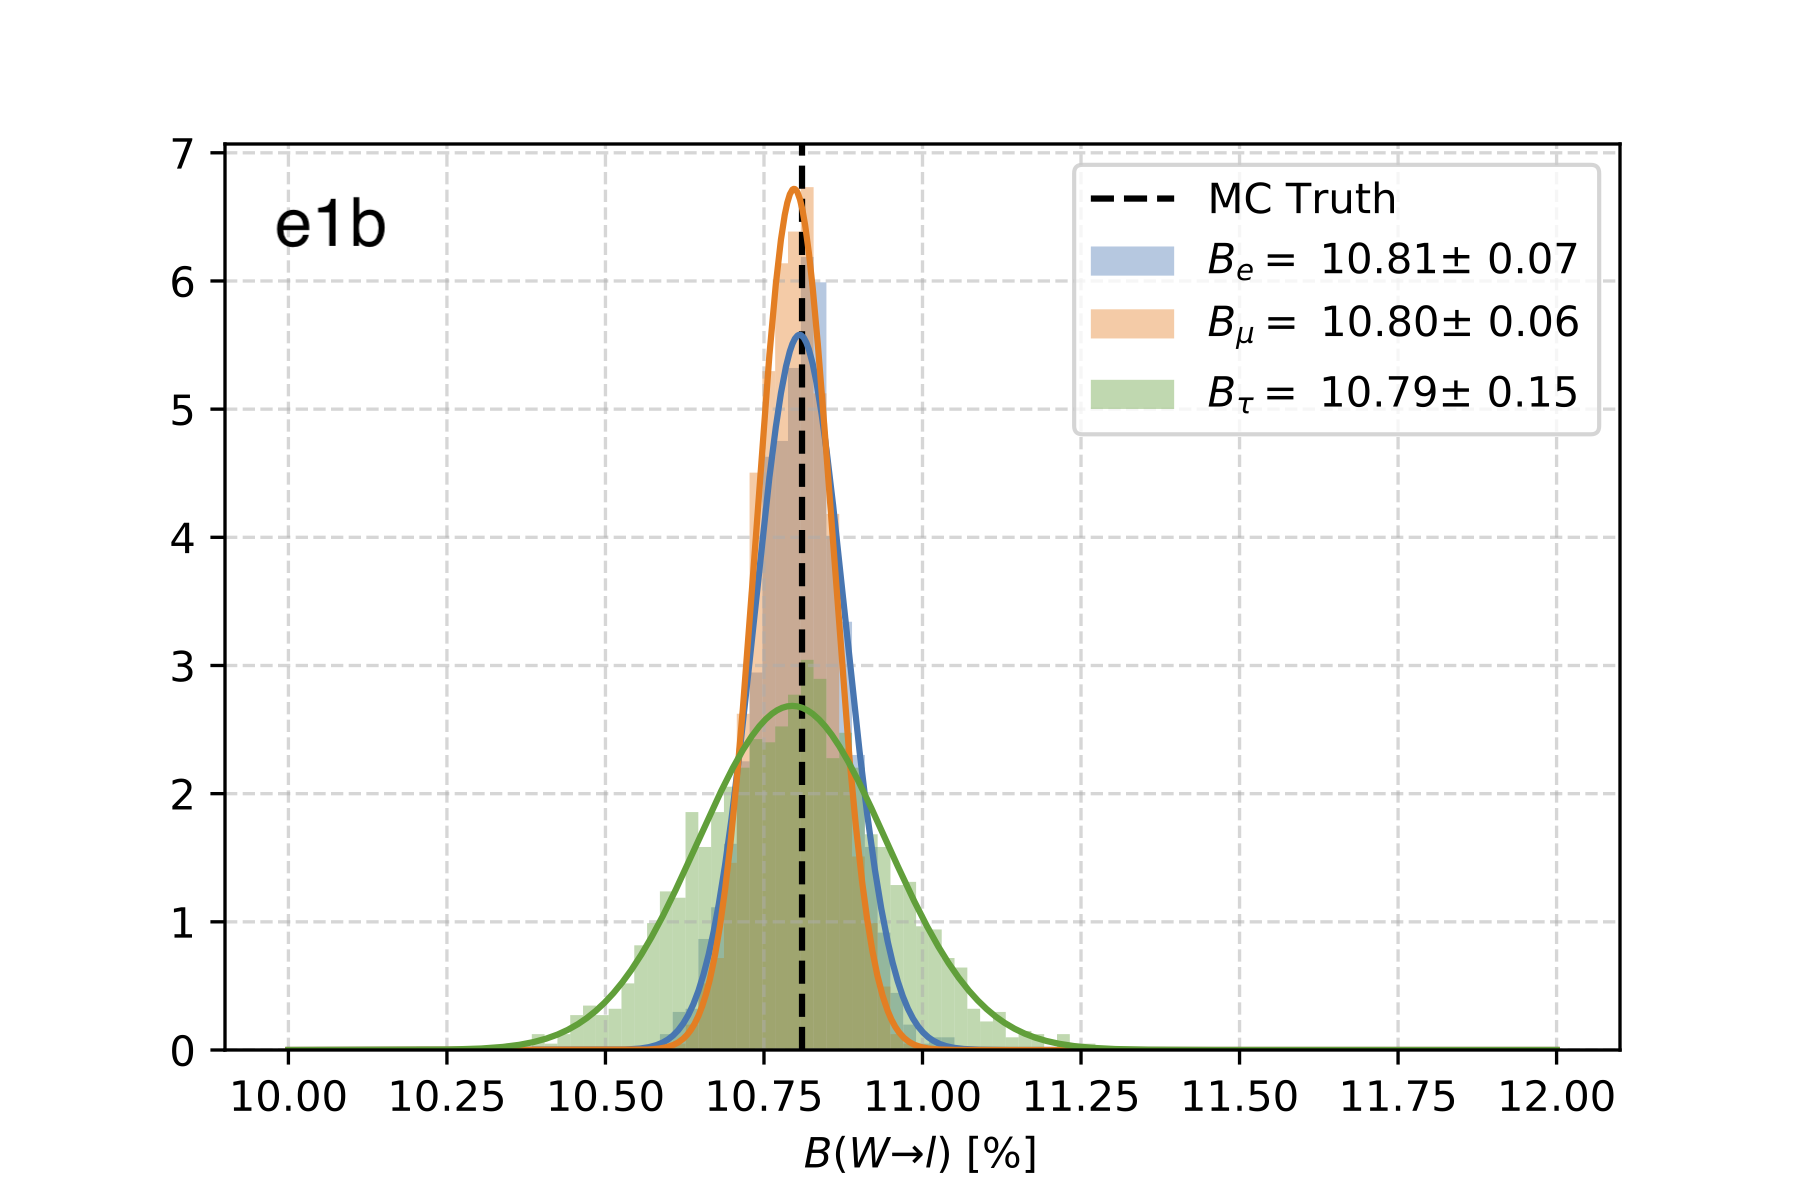
\includegraphics[width=7cm]{chapters/Analysis/sectionStatisticalAnalysis/figures/test_e1b.png}
    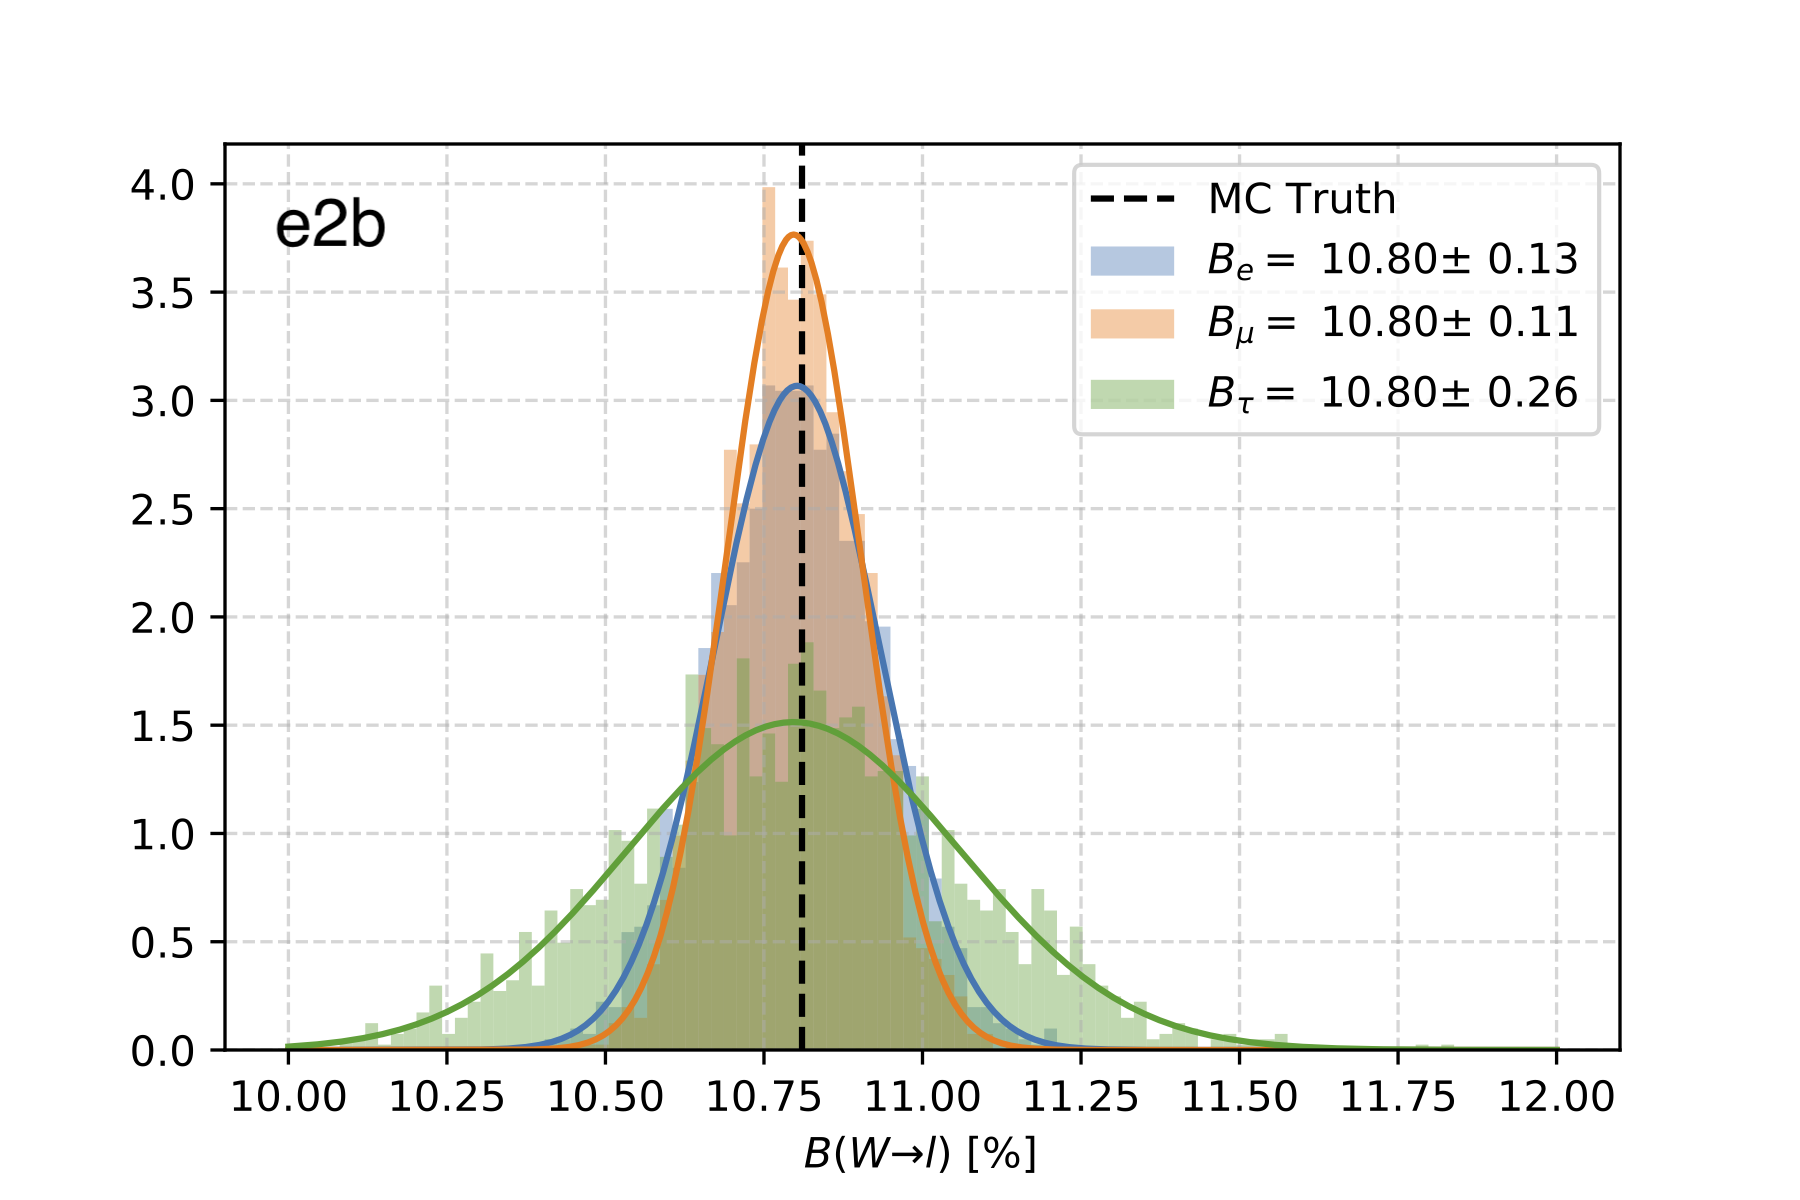
\includegraphics[width=7cm]{chapters/Analysis/sectionStatisticalAnalysis/figures/test_e2b.png}
    
    %--------------------------
    \caption{ Distribution of $\{\bwe,\bwm,\bwt\}$ extracted from two thousand toy datasets. }
    \label{fig:analysis:method:counting:test_toy}
\end{figure}


\FloatBarrier


% %%%%%%%%%%%%%%%%%%%%%%%%%%%%%%%%%%%%%%%%
% % 2. Extraction of Parameters
% %%%%%%%%%%%%%%%%%%%%%%%%%%%%%%%%%%%%%%%%
% \subsection{Extraction of Parameters}

% In counting analysis, branching fractions are extracted by solving a set of
% three quadratic equations, obtained by setting the expected normalized
% yields equal to the measured ones. The four measurements are performed independently 
% in four mutually exclusive regions based on the number of \PQb tags (1 or more than 2) 
% and trigger type (single electron or muon). Then these four measurements are combined based 
% on a $\chi^{2}$ minimization to obtain the final result.

% The four groups of channels and their yields
% are shown in figure~\ref{fig:signalRegion}.
% Channels using single-$\PGm$ or single-$e$ trigger are

% \begin{itemize}
%     \item single-$\PGm$ trigger : \cme, \cmm, \cmt, \cmh.
%     \item single-$e$ trigger : \cee, \cem, \cet, \ceh.
% \end{itemize}

% where \cem and \cme are mutually exclusive -- \cem channel
% requires fired e-trigger and $\pt^e > \pt^\PGm$, while \cme channel
% requires fired $\PGm$-trigger and $\pt^e < \pt^\PGm$. 

% Besides being formally different from the shape analysis, the thresholds
% of leptons $p^T$ and working point for the hadronic tau isolation are
% slightly different, as optimizations in counting. This results in slightly different signal
% acceptances. For the 8 channels under consideration, the signal efficiency determined from
% simulated $t\bar{t}$ and tW events are shown in
% tables \ref{efficencyTableMuon} and \ref{efficencyTableElectron}. 
% The efficiency matrices $\boldsymbol{E}$ of 
% included channels in the four categories are shown in Fig \ref{efficencyMatrix}.



% The normalized yields, which are inspired by the definition of branching
% fraction, is the ratio of one yield over the sum of all yields in the
% trigger category:


% \begin{itemize}
%     \item single-$\PGm$ trigger : 
%     $X_\Pe = \frac{n^{\PGm e}}{n^{\PGm e} + n^{\PGm \PGm} + n^{\PGm \PGt} + n^{\PGm \mathrm{h}}$, 
%     $X_\PGm = \frac{n^{\PGm \PGm}}{n^{\PGm e} + n^{\PGm \PGm} + n^{\PGm \PGt} + n^{\PGm h}}$, 
%     $X_\PGt = \frac{n^{\PGm \PGt}}{n^{\PGm e} + n^{\PGm \PGm} + n^{\PGm \PGt} + n^{\PGm h}}$,

%     \item single-$e$ trigger : 
%     $X_\Pe = \frac{n^{e e}}{n^{e e} + n^{e \PGm} + n^{e \PGt} + n^{e h}}$, 
%     $X_\PGm = \frac{n^{e \PGm}}{n^{e e} + n^{e \PGm} + n^{e \PGt} + n^{e h}}$, 
%     $X_\PGt = \frac{n^{e \PGt}}{n^{e e} + n^{e \PGm} + n^{e \PGt} + n^{e h}}$,
% \end{itemize}

% where $n^f \equiv N^f - \sum_{k\in bg} N^f_k $ is the yield of channel
% $f$ with background subtracted. Based on Eqn \ref{eqn:analysis:method:effMatrix:data_model}, the measured normalized yields
% $\{X_\Pe,X_\PGm,X_\PGt\}$ should equal to the calculation with
% efficiency $\boldsymbol{E}$ and branching fraction $\boldsymbol{B}$:

% \begin{equation} \label{quadEqA}
%     \begin{split}
%     X_e &= \frac{ \Eij^{\ctre}B^{ij} }{\Eij^{\ctre}B^{ij} + \Eij^{\ctrm}B^{ij} + \Eij^{\ctrt}B^{ij} + \Eij^{th}B^{ij}} \\
%     X_\PGm &= \frac{ \Eij^{\ctrm}B^{ij} }{\Eij^{\ctre}B^{ij} + \Eij^{\ctrm}B^{ij} + \Eij^{\ctrt}B^{ij} + \Eij^{th}B^{ij}} \\
%     X_\PGt &= \frac{ \Eij^{\ctrt}B^{ij} }{\Eij^{\ctre}B^{ij} + \Eij^{\ctrm}B^{ij} + \Eij^{\ctrt}B^{ij} + \Eij^{th}B^{ij}}
%     \end{split}
% \end{equation}



% % where $n^f \equiv N^f - \sum_{k\in bg} n^f_k $ is the yield of channel $f$ 
% % with background subtracted and three normalized yields, 
% % $\{r_\Pe,r_\PGm,r_\PGt\}$, are measured from data with background subtracted. 

% % Based on Eqn \ref{prediction}, the measured normalized yields $\{r_\Pe,r_\PGm,r_\PGt\}$ 
% % should equal to the calculation with efficiency $\boldsymbol{E}$ and branching fraction $\boldsymbol{B}$:




% where $t\in \{\PGm,e\}$ depends on the trigger category. Plugging in
% explicit form of $\boldsymbol{E}$ and $\boldsymbol{B}$ matrices in Eqn \ref{eqn:analysis:method:effMatrix:br_matrix} and Eqn \ref{eqn:analysis:method:effMatrix:eff_matrix}
% and unity condition of branching fraction $\bwh = 1- \bwe -
% \bwm - \bwt$, Eq \ref{quadEqA} can be written as a set of
% three quadratic equations with
% $\{\bwe,\bwm,\bwt\}$ as three unknowns.


% \begin{equation} \label{quadEqB}
%     \footnotesize
% 	\begin{split}
%         Q_e(\bwe,\bwm,\bwt) &=
%         c_{\Pe1} \bwe^2 + c_{\Pe2} \bwm^2 + c_{\Pe3} \bwt^2 + 
%         c_{\Pe4} \bwe\bwm + c_{\Pe5} \bwe\bwt + c_{\Pe6} \bwm\bwt +
%         c_{\Pe7} \bwe + c_{\Pe8} \bwm + c_{\Pe9} \bwt + c_{\Pe0} = 0 \\
%         %
%         Q_\PGm(\bwe,\bwm,\bwt) &= 
%         c_{\PGm 1} \bwe^2 + c_{\PGm 2} \bwm^2 + c_{\PGm 3} \bwt^2 + 
%         c_{\PGm 4} \bwe\bwm + c_{\PGm 5} \bwe\bwt + c_{\PGm 6} \bwm\bwt +
%         c_{\PGm 7} \bwe + c_{\PGm 8} \bwm + c_{\PGm 9} \bwt + c_{\PGm 0} = 0 \\
%         %
%         Q_\PGt(\bwe,\bwm,\bwt) &= 
%         c_{_\PGt1} \bwe^2 + c_{\PGt2} \bwm^2 + c_{\PGt3} \bwt^2 + 
%         c_{\PGt4} \bwe\bwm + c_{\PGt5} \bwe\bwt + c_{\PGt6} \bwm\bwt +
%         c_{\PGt7} \bwe + c_{\PGt8} \bwm + c_{\PGt9} \bwt + c_{\PGt0} = 0 
%     \end{split}
% \end{equation}

% where coefficients $c_{\Pei},c_{\PGm i},c_{\PGt i}$ are fully determined 
% by efficiency $\boldsymbol{E}$ and normalized yields $\{X_\Pe,X_\PGm,X_\PGt\}$,
% as are listed in table~\ref{quadcoeff}.

% \begin{table}[ht]
    \centering
   	\setlength{\tabcolsep}{0.4em}
    \renewcommand{\arraystretch}{1.5}
    \small
    
    \begin{tabular}{c|l}

    \hline
    $c_{l0}$ & $\Delta_{hh}$ \\
    \hline
    $c_{l1}$ & $\Delta_{ee}     - 2\Delta_{eh}   + \Delta_{hh}$ \\
    \hline
    $c_{l2}$ & $\Delta_{\mu\mu} - 2\Delta_{\mu h} + \Delta_{hh}$ \\
    \hline
    
    $c_{l3}$ & $   b^\tau_e   b^\tau_e   \Delta_{\tau_e   \tau_e}  
    			 + b^\tau_\mu b^\tau_\mu \Delta_{\tau_\mu \tau_\mu}
                 + b^\tau_h   b^\tau_h   \Delta_{\tau_h   \tau_h}
                 
                 + 2 b^\tau_e   b^\tau_\mu \Delta_{\tau_e   \tau_\mu} 
    		     + 2 b^\tau_e   b^\tau_h   \Delta_{\tau_e   \tau_h}   
    		     + 2 b^\tau_\mu b^\tau_h   \Delta_{\tau_\mu \tau_h} - $ \\
                 
             & $   2 b^\tau_e   \Delta_{e   \tau_h}
                 - 2 b^\tau_\mu \Delta_{\mu \tau_h}
                 - 2 b^\tau_h   \Delta_{h.  \tau_h} 
                 + \Delta_{hh} $ \\

    \hline
    $c_{l4}$ & $2\Delta_{e\mu} - 2\Delta_{eh} -2\Delta_{\mu h} +2\Delta_{hh}$  \\
    \hline
    $c_{l5}$ & $  2b^\tau_e   \Delta_{e \tau_e} 
    			+ 2b^\tau_\mu \Delta_{e \tau_\mu}
                + 2b^\tau_h   \Delta_{e \tau_h}
                - 2b^\tau_e   \Delta_{\tau_e   h} 
    			- 2b^\tau_\mu \Delta_{\tau_\mu h}
                - 2b^\tau_h   \Delta_{\tau_h   h} 
                - 2\Delta_{eh}   + 2 \Delta_{hh} $ \\
        
    \hline            
    $c_{l6}$ & $  2b^\tau_e   \Delta_{\mu \tau_e} 
    			+ 2b^\tau_\mu \Delta_{\mu \tau_\mu}
                + 2b^\tau_h   \Delta_{\mu \tau_h}
                - 2b^\tau_e   \Delta_{\tau_e   h} 
    			- 2b^\tau_\mu \Delta_{\tau_\mu h}
                - 2b^\tau_h   \Delta_{\tau_h   h} 
                - 2\Delta_{\mu h}   + 2 \Delta_{hh} $ \\
    \hline            
    $c_{l7}$ & $ 2\Delta_{eh}      - 2 \Delta_{hh} $ \\
    \hline
    $c_{l8}$ & $ 2\Delta_{\mu h}   - 2 \Delta_{hh}$ \\
    \hline
    $c_{l9}$ & $  2b^\tau_e   \Delta_{\tau_e   h} 
                 + 2b^\tau_\mu \Delta_{\tau_\mu h} 
                 + 2b^\tau_h   \Delta_{\tau_h   h} 
                 - 2 \Delta_{hh}$ \\
    \hline
    \hline
    where  & $ \Delta \equiv E^{tl} - X_l \times ( E^{te} + E^{t\mu} + E^{t\tau} + E^{th} )$ \\
           & $l=e,\mu,\tau$ and $t=e(\mu)$ if using single-$e$ (signle-$\mu$) trigger\\
    \hline
    
	\end{tabular}
    
\caption{ Coefficients of quadratic equations in terms of E and X. In the table, $l=e,\mu,\tau$ and $t=\mu,e$ for single-$\mu$ and single-$e$ trigger respectively.  }
\label{quadcoeff}
    
\end{table}


% In the $\{\bwe,\bwm,\bwt\}$ parameter space, 
% equation~\ref{quadEqB} represents three hyperbolic planes, intersection 
% of which is the solution of desired branching fractions, as is shown
% in figure~\ref{visualize}.


% \begin{figure}[ht]
%     \centering
%     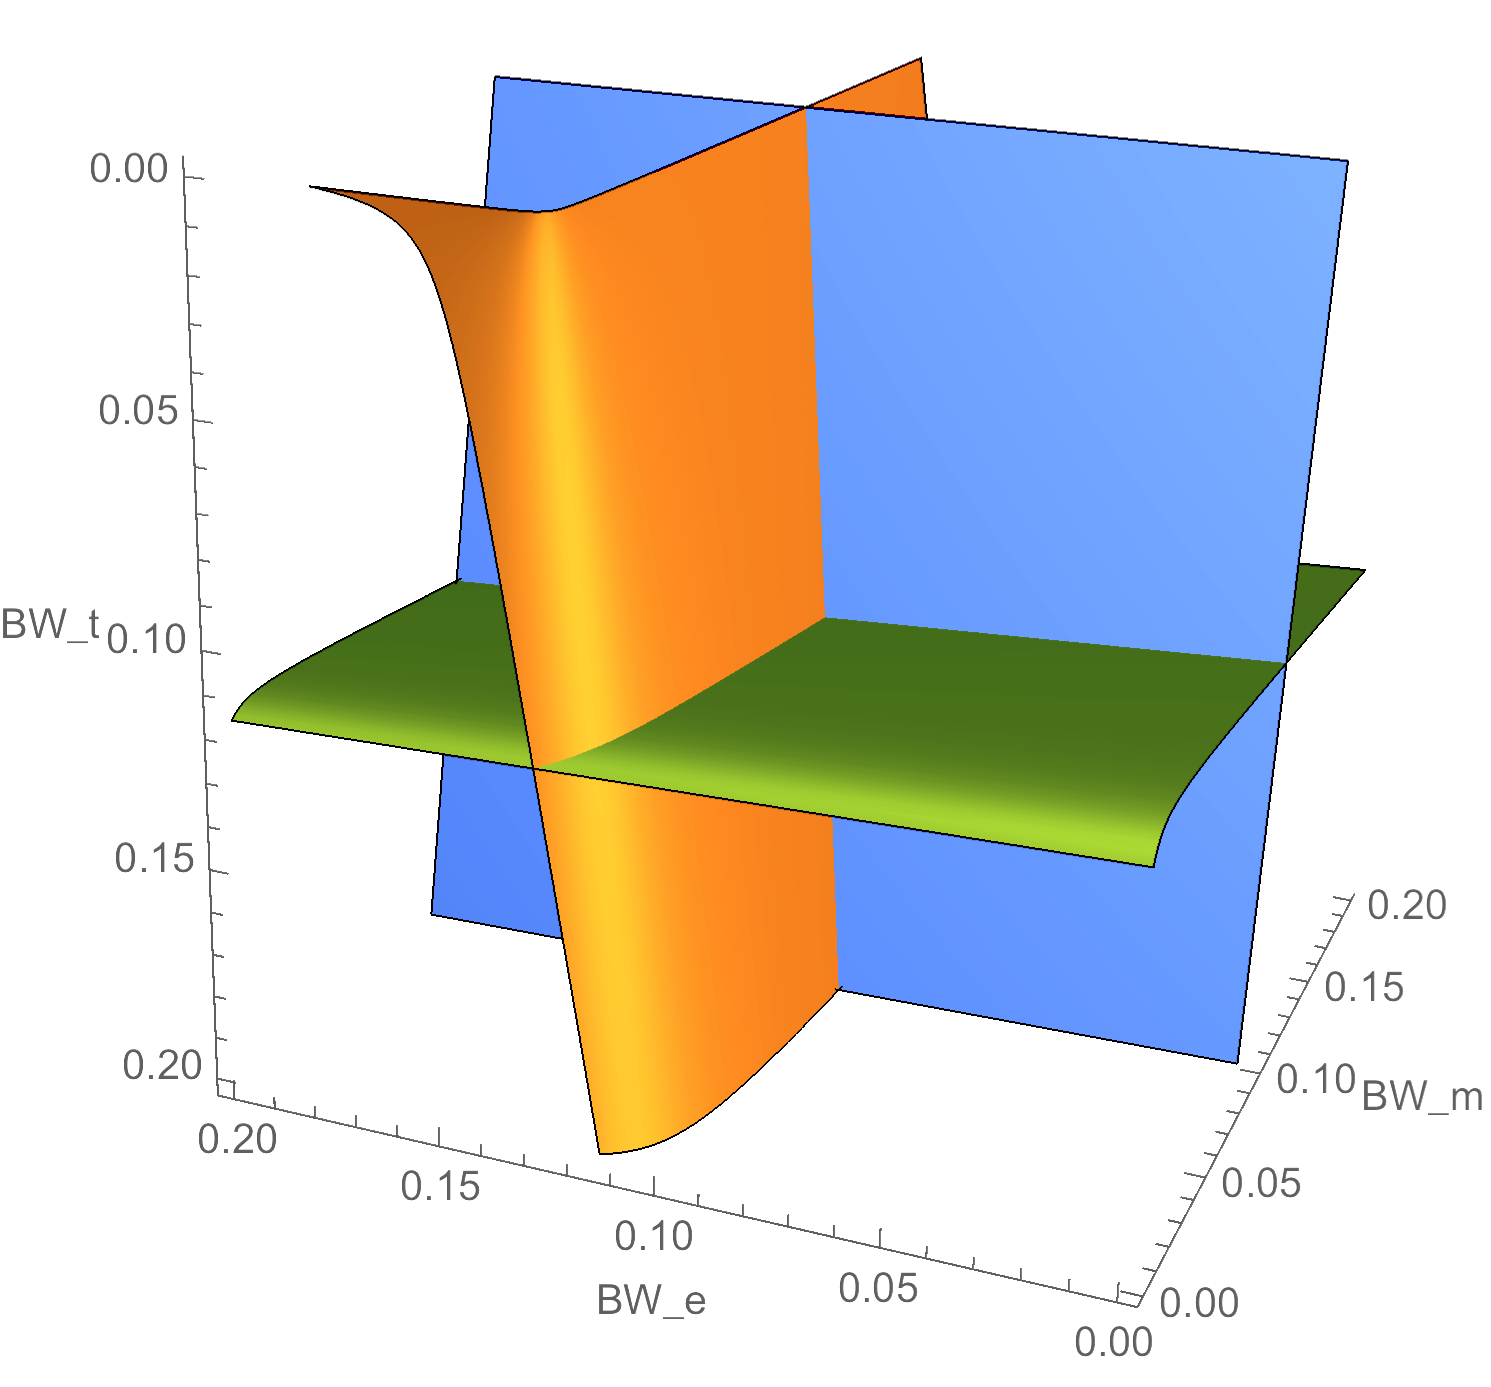
\includegraphics[width=7cm]{chapters/Analysis/sectionStatisticalAnalysis/figures/visual.png}
    
%     %--------------------------
%     \caption{Visualization of Eq \ref{quadEqB} in the
%     $\{\bwe,\bwm,\bwt\}$ parameter space. Each
%     equation in Eq \ref{quadEqB} is a hyperbolic plane, while their
%     intersection is the solution Eq \ref{quadEqB}. Mathematically, there
%     are 8 possible solutions. However, only one solution is physical,
%     located with $\beta \in (0,1) $. }
%     \label{visualize}
% \end{figure}

% % This approach analytically obtains the coefficient $c_{ij}$ in 
% % Eq \ref{quadEqB} from efficiency matrix $\boldsymbol{E}$ and measured 
% % normalized yields $\{X_\Pe,X_\PGm,X_\PGt\}$. Then it numerically
% % solves the branching fractions $\{\bwe,\bwm,\bwt\}$,
% % using a modification of the Powell hybrid method as implemented in MINPACK-Scipy. 

% \begin{equation} 
%     \left [
%     \begin{tabular}{c}
% 	    $\bwe$ \\
% 	    $\bwm$ \\
% 	    $\bwt$
%     \end{tabular}
%     \right ]
%     = Solution
%     \left [
%     \begin{tabular}{c}
% 	    $Q_e    (\bwe,\bwm,\bwt) = 0$ \\
% 	    $Q_\PGm  (\bwe,\bwm,\bwt) = 0$ \\
% 	    $Q_\PGt (\bwe,\bwm,\bwt) = 0$
%     \end{tabular}
% \right ]
% \end{equation}

% \FloatBarrier

%%%%%%%%%%%%%%%%%%%%%%%%%%%%%%%%%%%%%%%%
% 3. Test of Parameters Extraction
%%%%%%%%%%%%%%%%%%%%%%%%%%%%%%%%%%%%%%%%
% \subsection{Test of Parameters Extraction}






% \begin{quote}
    
%     After establishing parameter extraction, we perform a closure test using 
%     signal MC samples. As is described above, the input of parameter extraction 
%     is data yields with background subtracted $n=N_{data} - N_{mc,bg}$. 
%     But here for testing purpose, we replace $n=N_{data} - N_{mc,bg}$ with $N_{mc,sg}$ as the input,
%     as is given in Eqn \ref{eqn:testinput}.
%     The pass of the test is that parameter extraction 
%     gives back branching fraction assumed in the MC generator, which is $10.80\%$.
    
    
%     \begin{equation}
%     	n=N_{mc,sg}\pm \sqrt{N_{mc,sg}}
%     	\label{eqn:testinput}
%     \end{equation}
    
%     where $N_{mc,sg}$ comes from tt and tW MC sample normalized to luminosity. 
%     It is uncertainty is assumed as a Gaussian error with width $\sqrt{N_{sg}}$, 
%     so as to estimate the expected statistical uncertainty of data.
%     The extracted branching fraction is listed in Table \ref{test_ana}.

% \end{quote}



% \begin{table}[ht]
%     \centering
% 	\begin{tabular}{l|ccc}
%     \hline
%           	 & $\bwe$             &   $\bwm$       	 & 	  $\bwt$   	 \\
%     MC Assumption  & 10.80 		 &  10.80 		 	 & 	  10.80     	 \\
%     \hline
%   	$\PGm-1b$ &   10.802$\pm$0.058  &   10.807$\pm$0.053  &    10.808$\pm$0.127 \\
%   	$\PGm-2b$ &   10.802$\pm$0.103  &   10.807$\pm$0.092  &    10.808$\pm$0.216 \\
%   	$e-1b$   &   10.804$\pm$0.073  &   10.797$\pm$0.059  &    10.794$\pm$0.152 \\
%   	$e-2b$   &   10.805$\pm$0.130  &   10.797$\pm$0.104  &    10.794$\pm$0.263 \\
%     \hline
% 	\end{tabular}
	
% 	%--------------------------
%     \caption{Branching fraction extracted from signal MC. The 
%     uncertainty is calculated by error propagation. The small 
%     deviation from MC assumption is resulted by the difference 
%     value of $Br(\PGt \to e)$ and $Br(\PGt \to \PGm)$ in MC and in 
%     extractor. The extractor uses 0.1773,0.1731 respectively, while 
%     the MC assumption of tau decay needs to be found in generator 
%     cards. 
%     }
%     \label{test_ana}
% \end{table}



% In addition, to test the error propagation, we generate two thousand toy experiments, 
% each of which variates the yield $n=N_{sg}$ by $\sqrt{N_{sg}}$.
% The width of distribution of toys is consistent with uncertainty 
% from error propagation list in the Table \ref{test_ana}.
% Also as expected, the center of distribution of toys is consistent with
% the assumed branching fraction in the MC generator.






% Finally, the branching fractions obtained in all four categories are combined:

% \begin{equation}
% 	\beta_i = \frac{ \sum_{cat} \beta_i^{cat} / \sigma^2_{\beta_i^{cat}}}{\sum_{cat} 1 / \sigma^2_{\beta_i^{cat}}} ,
%     \qquad
%     \sigma^2_{\beta_i} = \frac{1}{\sum_{cat} 1 / \sigma^2_{\beta_i^{cat}} }
% \end{equation}

% where $i = e,\PGm,\PGt$ and categories are single electron or muon trigger with 1 or 2 \PQb jets, $cat \in \{\PGm \text{-} 1b,\PGm \text{-} 2b,e \text{-} 1b,e \text{-} 2b \}$

